 \section{Application to air pollution forecasting}

   The World Health Organization estimated that approximately seven million people die every year due to air pollution \cite{CityofCapeTown2024}. To manage levels of air pollution, the City of Cape Town has built eleven air quality monitoring (AQM) stations in Cape Town. These stations collect data on particulate matter 10 $(\text{PM}_{10})$, particulate matter 2.5 $(\text{PM}_{2.5})$, sulphur dioxide $(\text{SO}_{2})$, nitrogen dioxide $(\text{NO}_{2})$, ozone $(\text{O}_{3})$, hydrogen sulphide $(\text{H}_{2}\text{S})$, carbon monoxide $(\text{CO})$, benzene $(\text{C}_{6}\text{H}_{6})$, and lead $(\text{Pb})$ \cite{CityofCapeTown2024}. Air pollution data for Cape Town can be found on the City of Cape Town open data portal \cite{CityofCapeTown2015}. The goal of this analysis is to understand the range of ordinary values for air pollutants. This would serve as an indicator for high levels of air pollutants, and actions can be taken to mitigate the situation. We consider only short-term forecasts because prediction using Gaussian processes is computationally expensive.
      
   \subsection{Description of the data}

      The Table View station was chosen for this project. This is because it had the fewest missing observations. The data consist of our response variable, nitrogen dioxide $(\mu g / m^3)$, and explanatory variables, sulphur dioxide $(\mu g / m^3)$, particulate matter 10 $(\mu g / m^3)$, and wind speed $(m/s)$ from 01/01/2019 to 31/12/2019, measured hourly at the Table View station. Nitrogen dioxide is chosen as the response variable because it is the most correlated with the other variables. It would be easier to predict nitrogen dioxide using the other variables as covariates.

      \begin{table}[ht]
         \centering
         \begin{tabular}{lrrrrrrrrr}
            \toprule
                  & Min. & 1st Qu. & Median & Mean   & SD     & 3rd Qu. & Max.  & \#Tot. & \#NA. \\
            \midrule
            NO2     & 0.0  & 5.0     & 9.0    & 12.729 & 10.724 & 17.0    & 113.0 & 8003   & 734   \\
            PM10    & 0.0  & 12.0    & 17.0   & 19.824 & 12.302 & 24.0    & 158.0 & 8439   & 298   \\
            SO2     & 0.0  & 2.0     & 3.0    & 6.202  & 11.299 & 5.0     & 142.0 & 8099   & 638   \\
            Speed   & 0.5  & 2.3     & 3.6    & 3.735  & 1.710  & 4.9     & 11.2  & 7819   & 918   \\
            \bottomrule
         \end{tabular}
         \caption{Summary statistics of the air quality dataset from 01/01/2019 to 31/12/2019 measured hourly.}
         \label{tab:summary_stats}
      \end{table}

      All variables in this data set are non-negative. There are many observations missing. Gaussian processes cannot handle missing data directly. To mitigate this, we consider the window of the data set with the longest sub-sequence of no missing values. This window is from 15/02/2019 at 23:00:00 to 06/03/2019 at 23:00:00. This is a total of 456 hours or 19 days. This is the data set that is going to be used for training and testing purposes of this analysis.

      \begin{table}[ht]
      \centering
      \begin{tabular}{lrrrrrrrrr}
         \toprule
               & Min. & 1st Qu. & Median & Mean  & SD    & 3rd Qu. & Max. & \#Tot. & \#NA. \\
         \midrule
         NO2    & 2.0  & 6.0     & 9.0    & 10.348 & 5.607 & 13.0    & 40.0 & 457    & 0     \\
         PM10   & 4.0  & 12.0    & 16.0   & 17.888 & 9.606 & 22.0    & 83.0 & 457    & 0     \\
         SO2    & 1.0  & 2.0     & 3.0    & 6.510  & 12.181 & 4.0    & 128.0 & 457   & 0     \\
         Speed  & 0.7  & 2.4     & 3.5    & 3.575  & 1.397 & 4.6     & 7.2  & 457    & 0     \\
         \bottomrule
      \end{tabular}
      \caption{Summary statistics of the air quality dataset from 15/02/2019 at 23:00:00 to 06/03/2019 at 23:00:00 measured hourly.}
      \label{tab:summary_stats2}
      \end{table}

      \subsubsection{Exploratory data analysis}

         \begin{figure}[H]
            \centering
            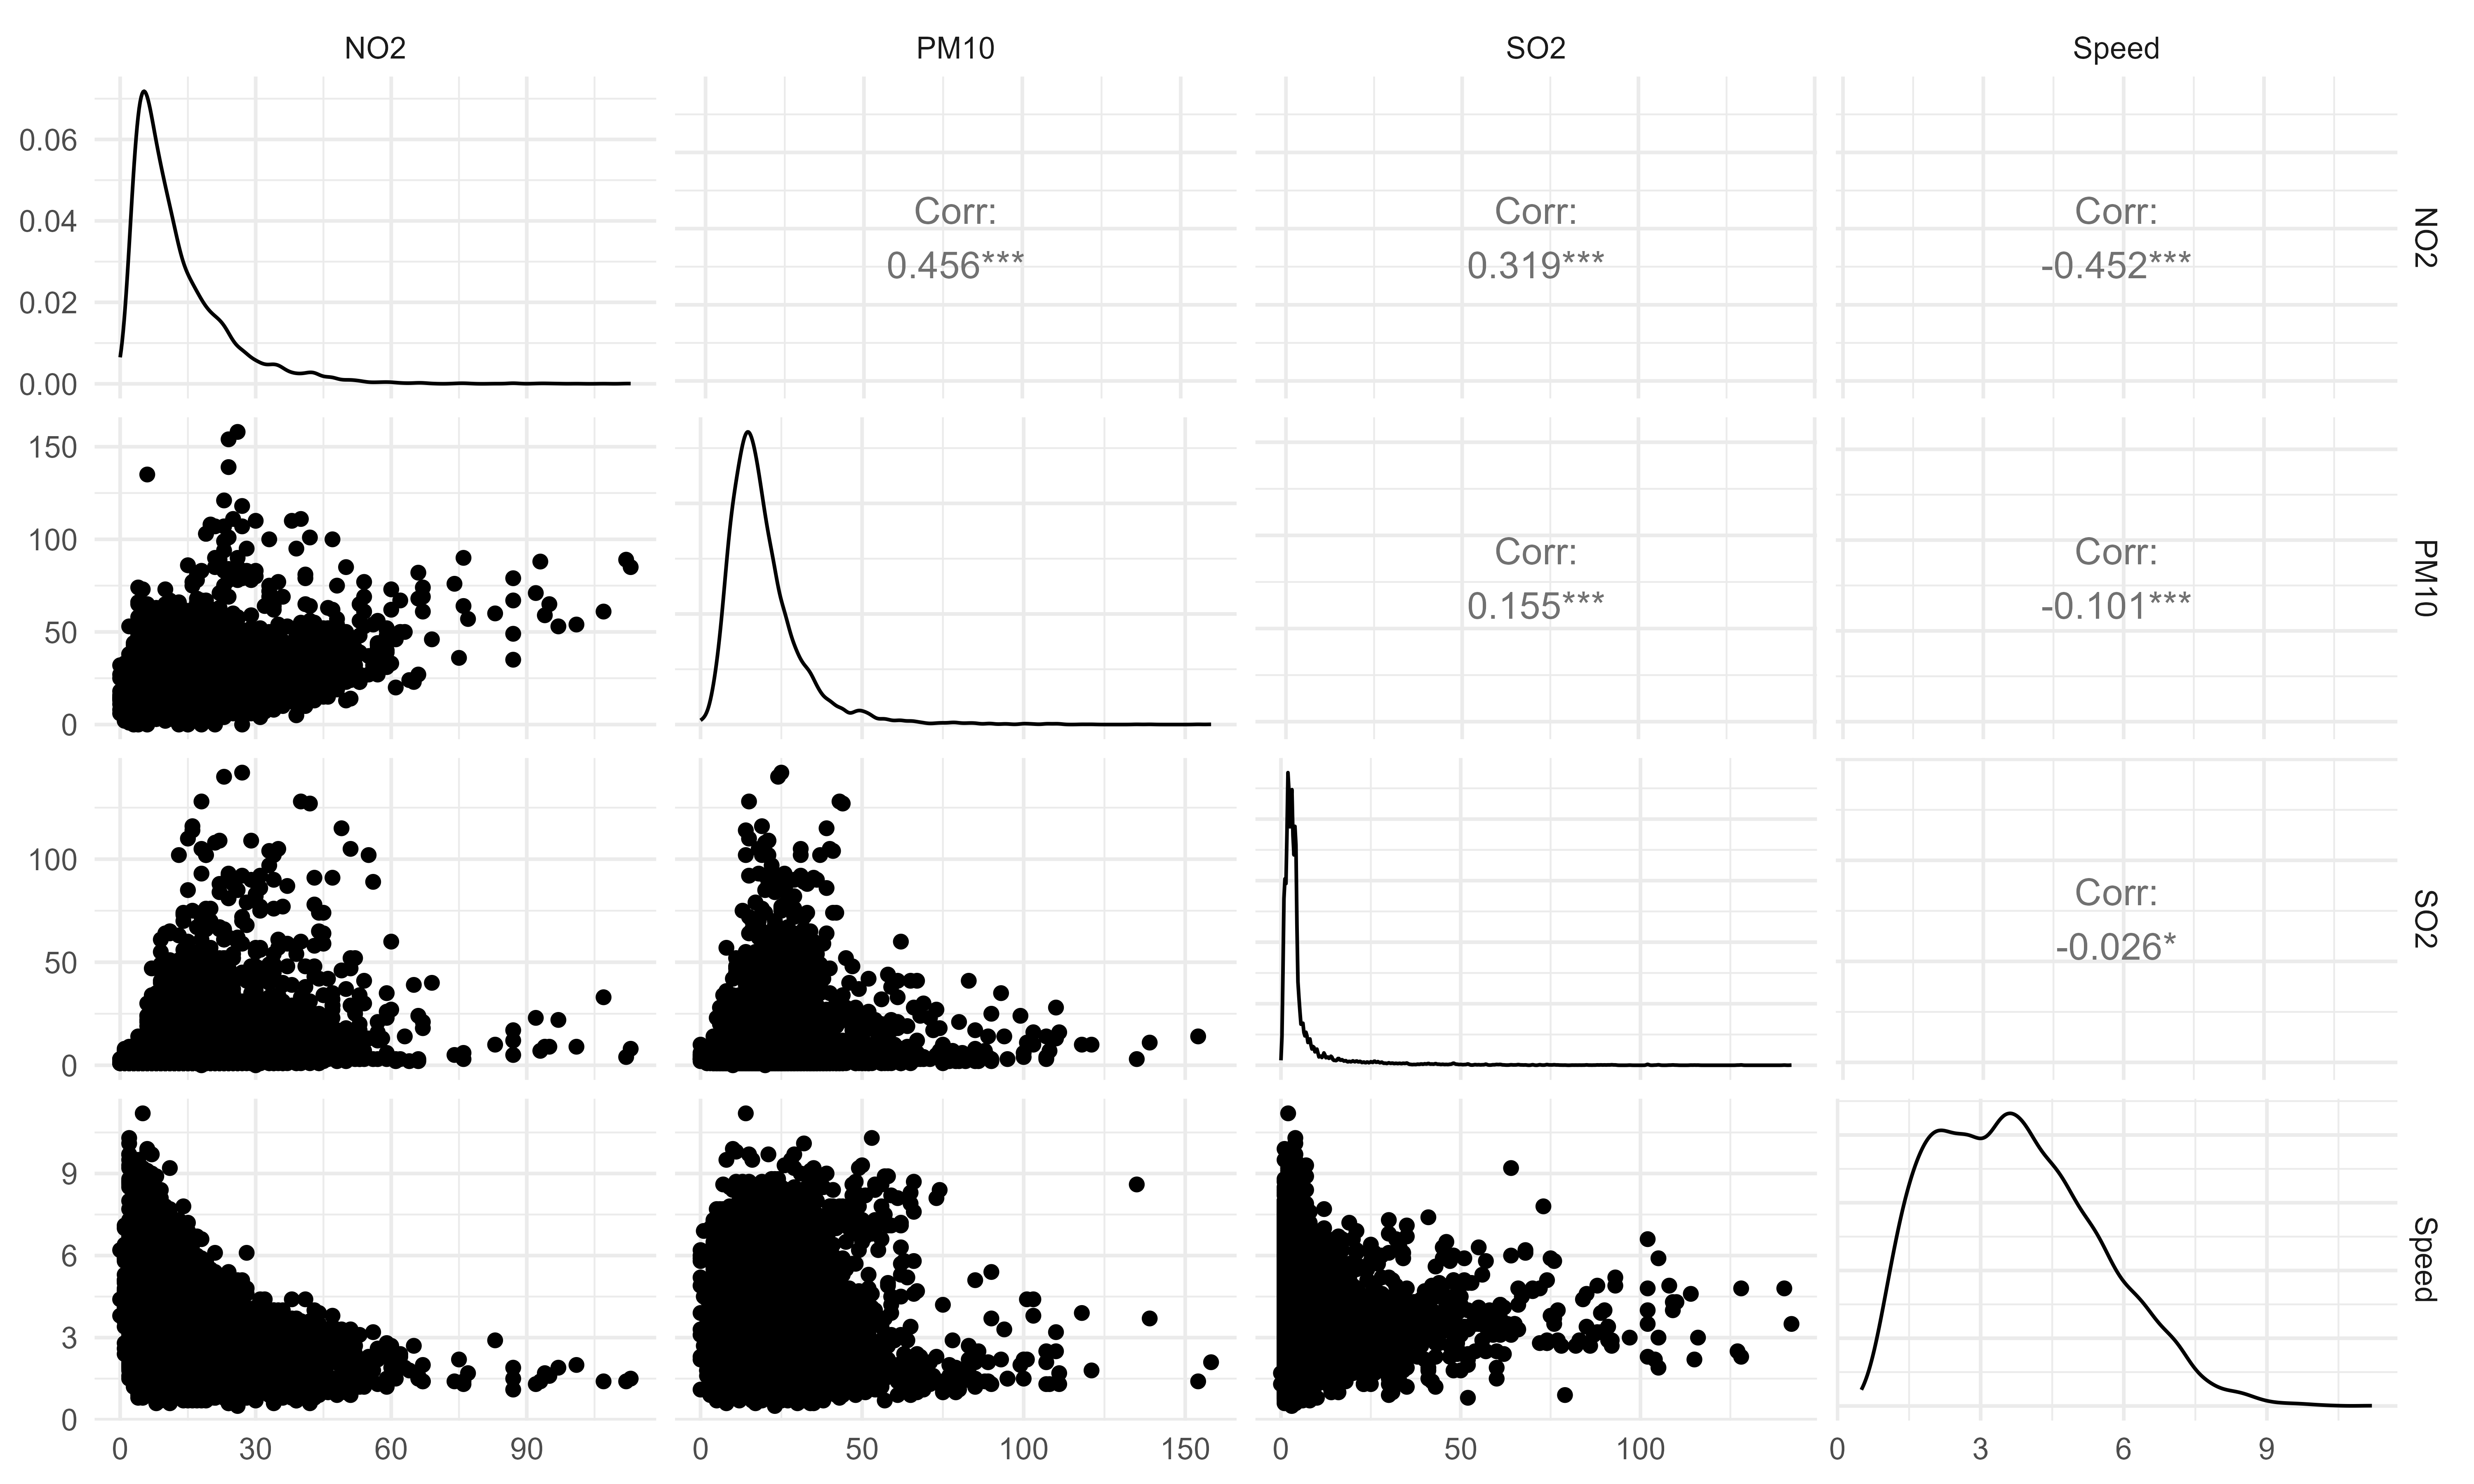
\includegraphics[width=0.48\linewidth]{../images/extracted_data_pairsplot.png}
            \caption{\textit{Pairs plot of the air quality dataset from 01/01/2019 to 31/12/2019 measured hourly.}}
         \end{figure}

         Our response variable $\text{NO}_{2}$ appears to be moderately positively correlated with $\text{PM}_{10}$ and $\text{SO}_{2}$, and moderately negatively correlated with Speed. These are not ideal explanatory variables since we typically would like them to be strongly correlated with the response variable. The explanatory variables are weakly correlated with one another, whether it be a positive or a negative correlation. This is ideal since some models do not work well with correlated explanatory variables, often leading to unstable point estimates and inflated standard errors.

         \begin{figure}[H]
            \centering
            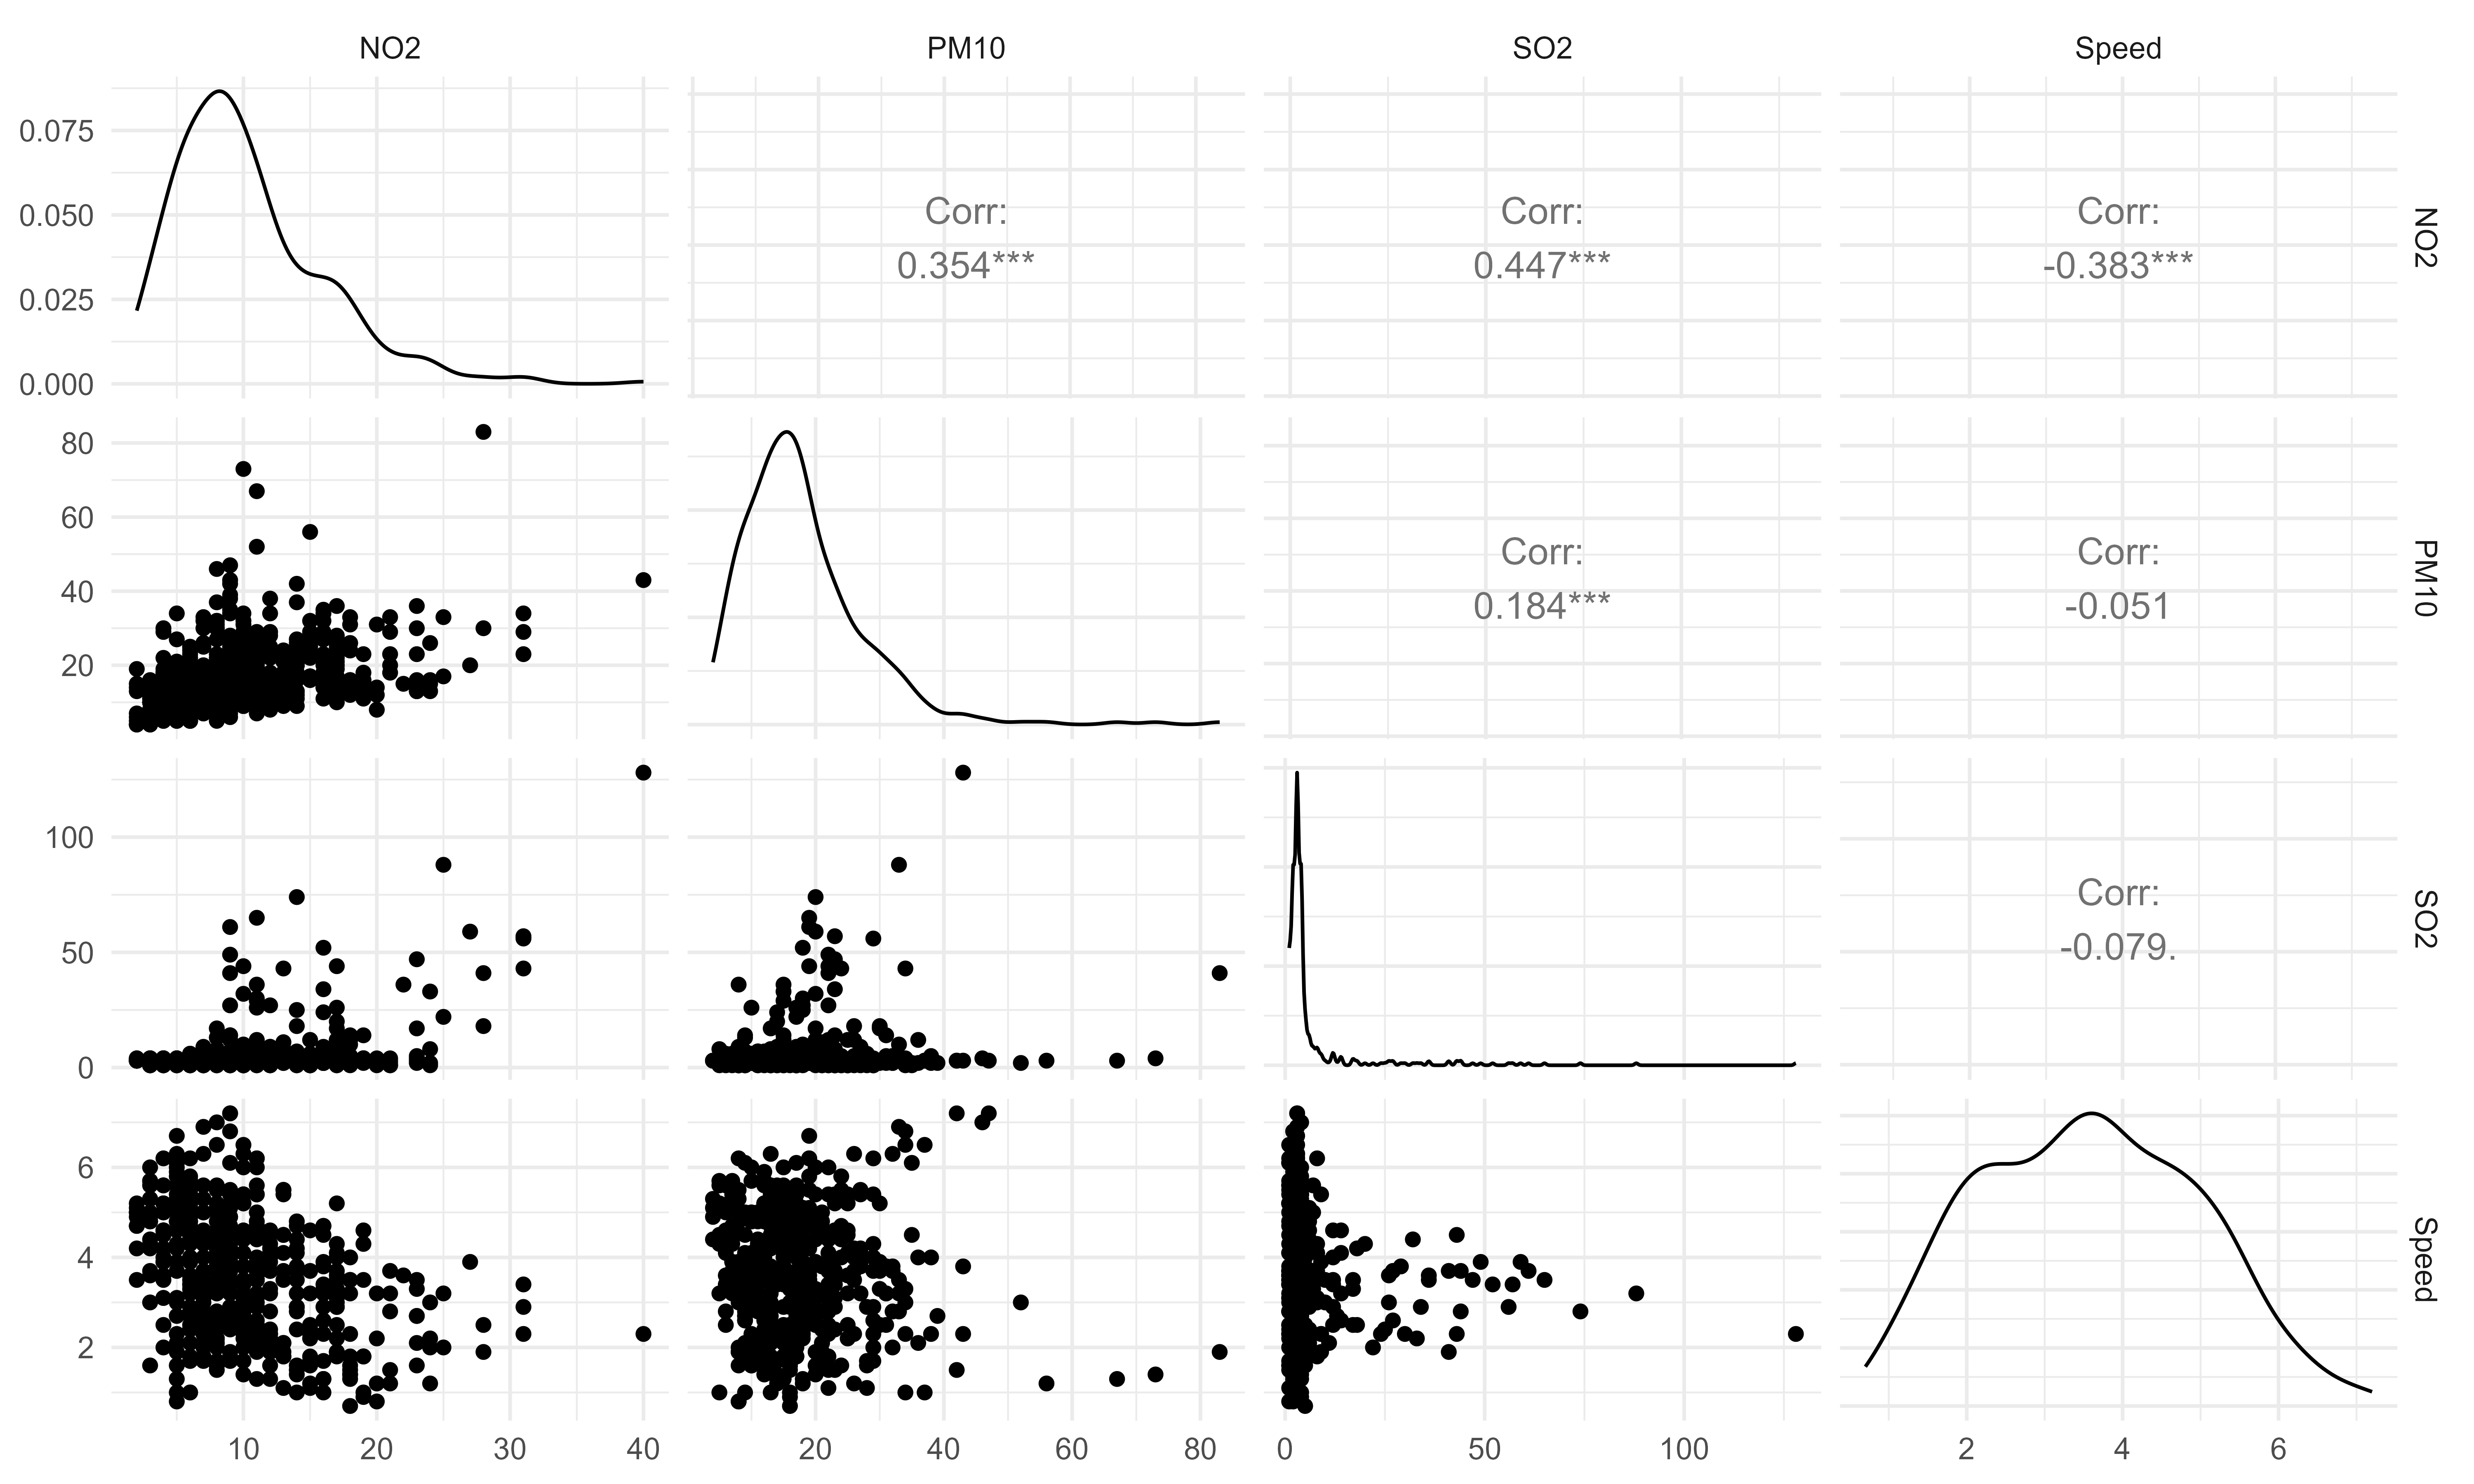
\includegraphics[width=0.48\linewidth]{../images/subset_data_pairsplot.png}
            \caption{\textit{Pairs plot of the air quality dataset from 01/01/2019 to 31/12/2019 measured hourly.}}
         \end{figure}

         \begin{figure}[H]
            \centering
            \begin{subfigure}{0.48\linewidth}
               \centering
               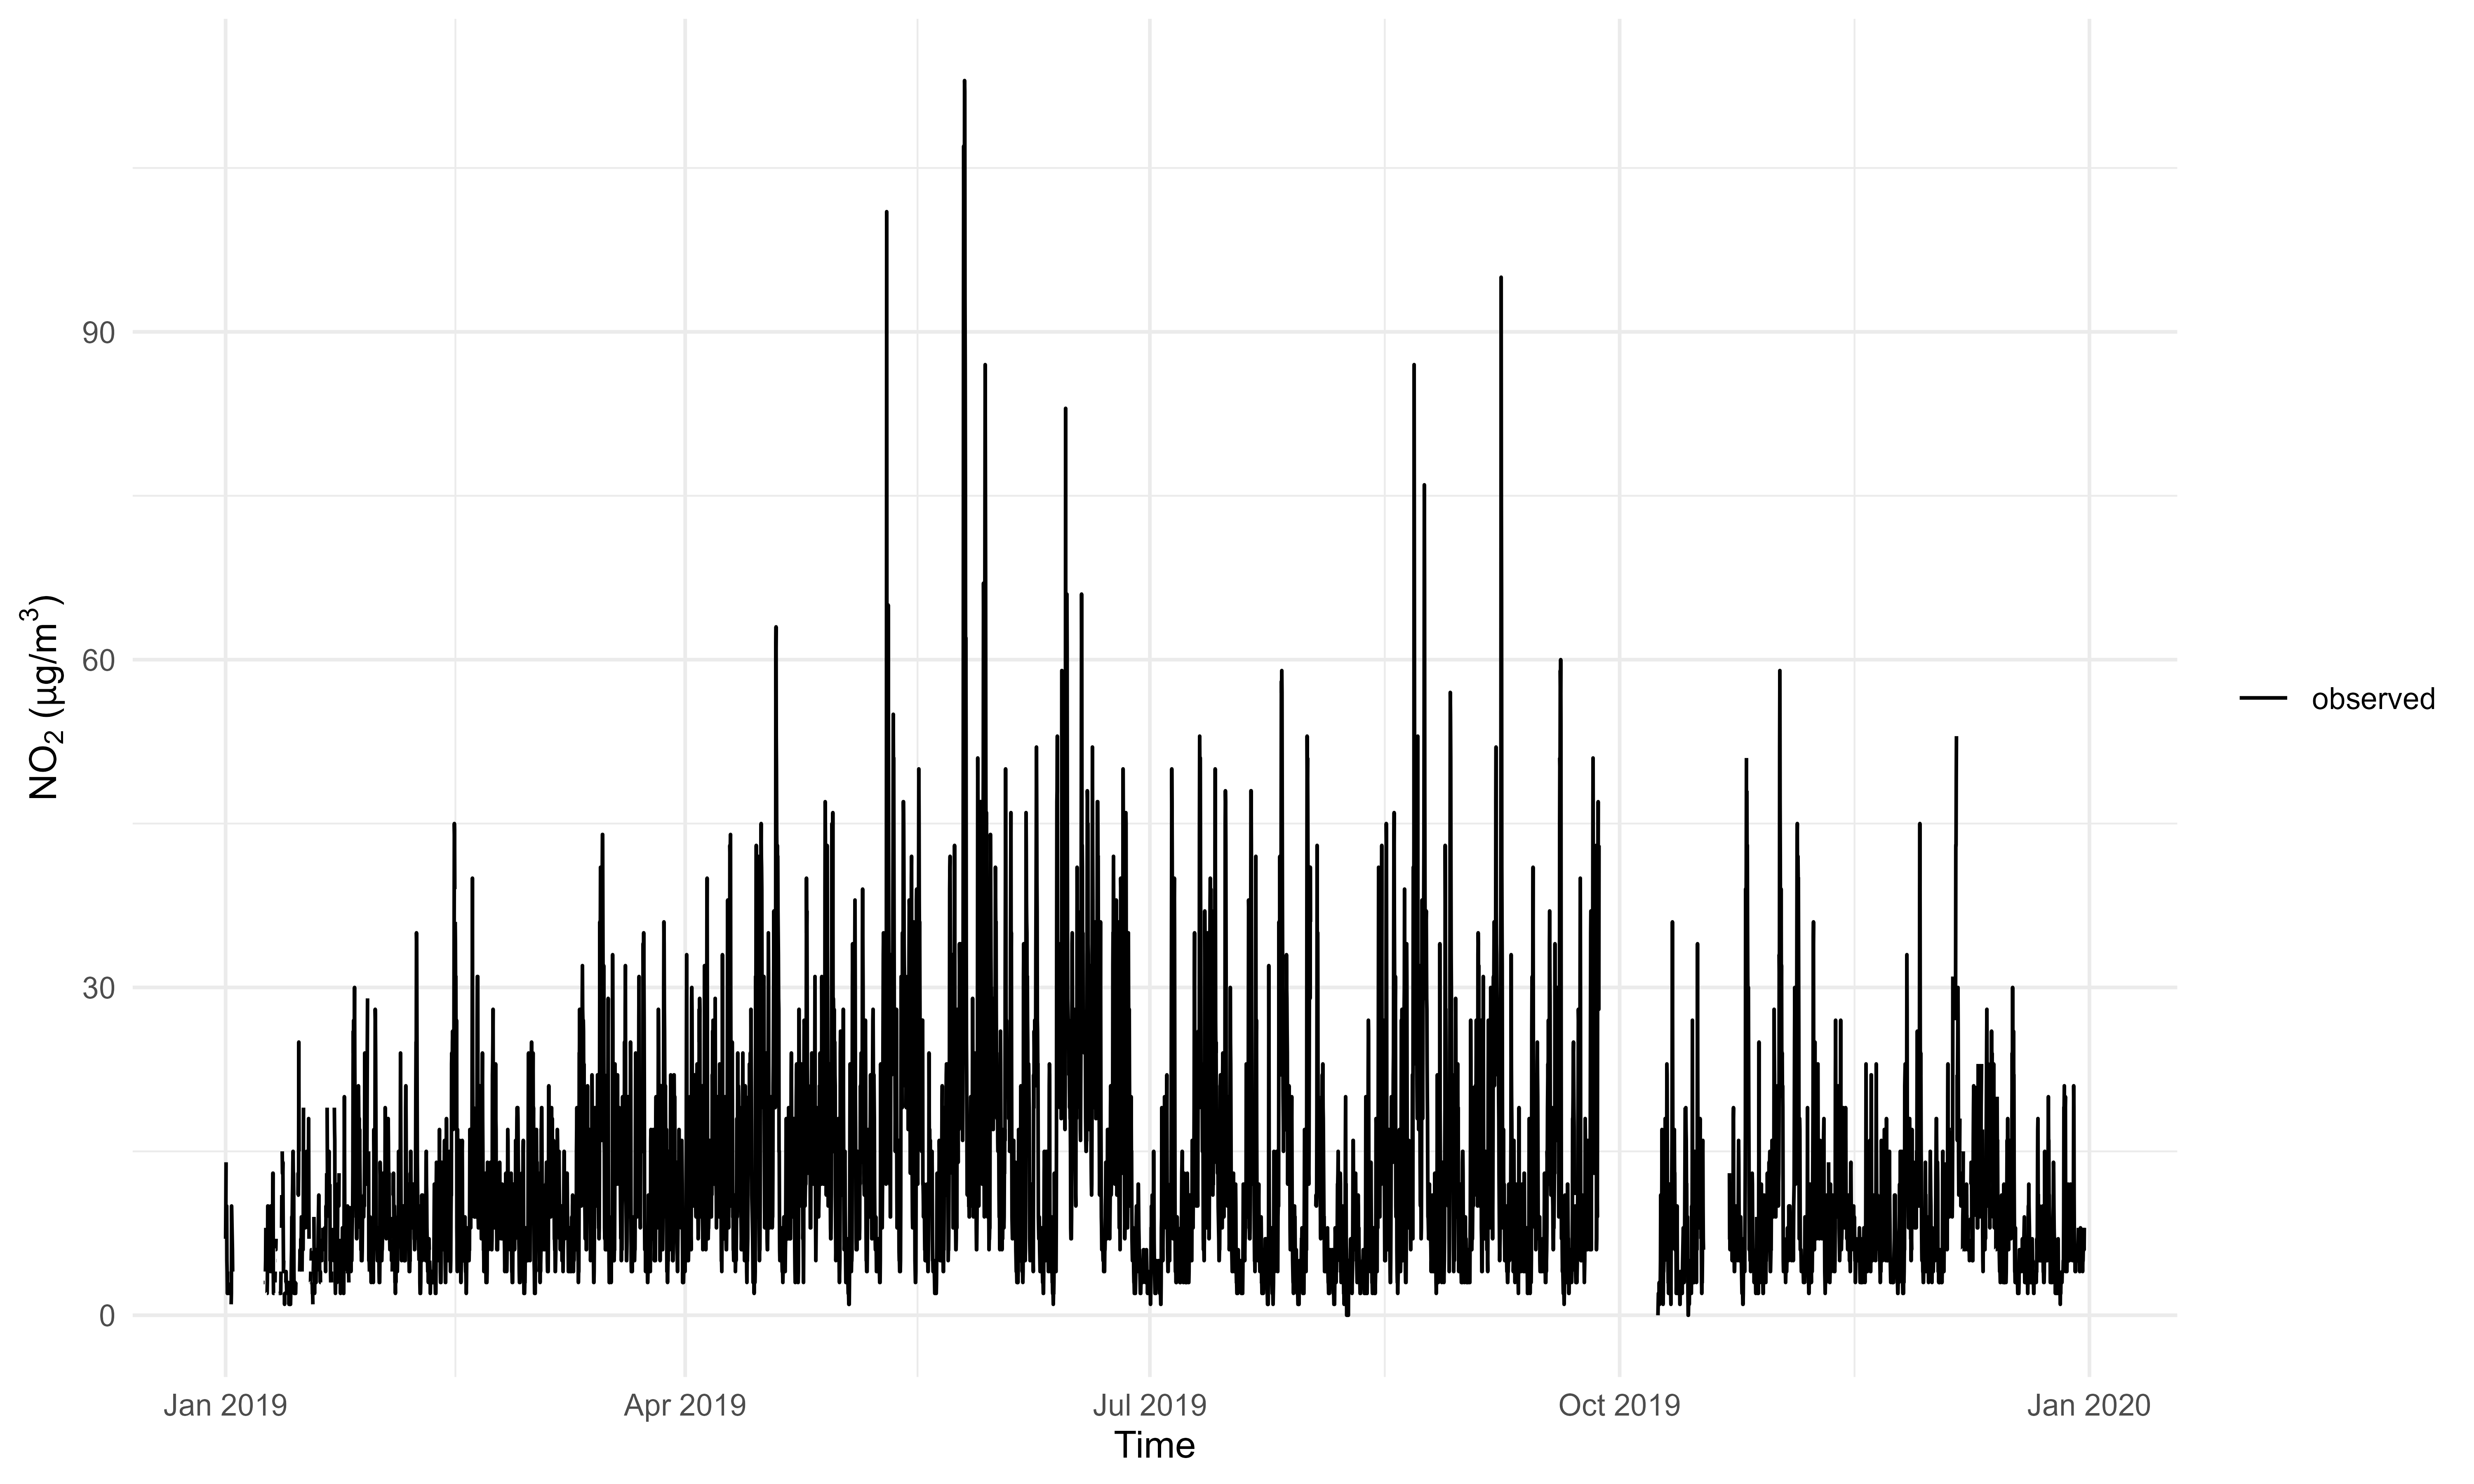
\includegraphics[width=\linewidth]{../images/extracted_data_no2.png}
            \caption{Nitrogen dioxide}
            \end{subfigure}
            \hfill
            \begin{subfigure}{0.48\linewidth}
               \centering
               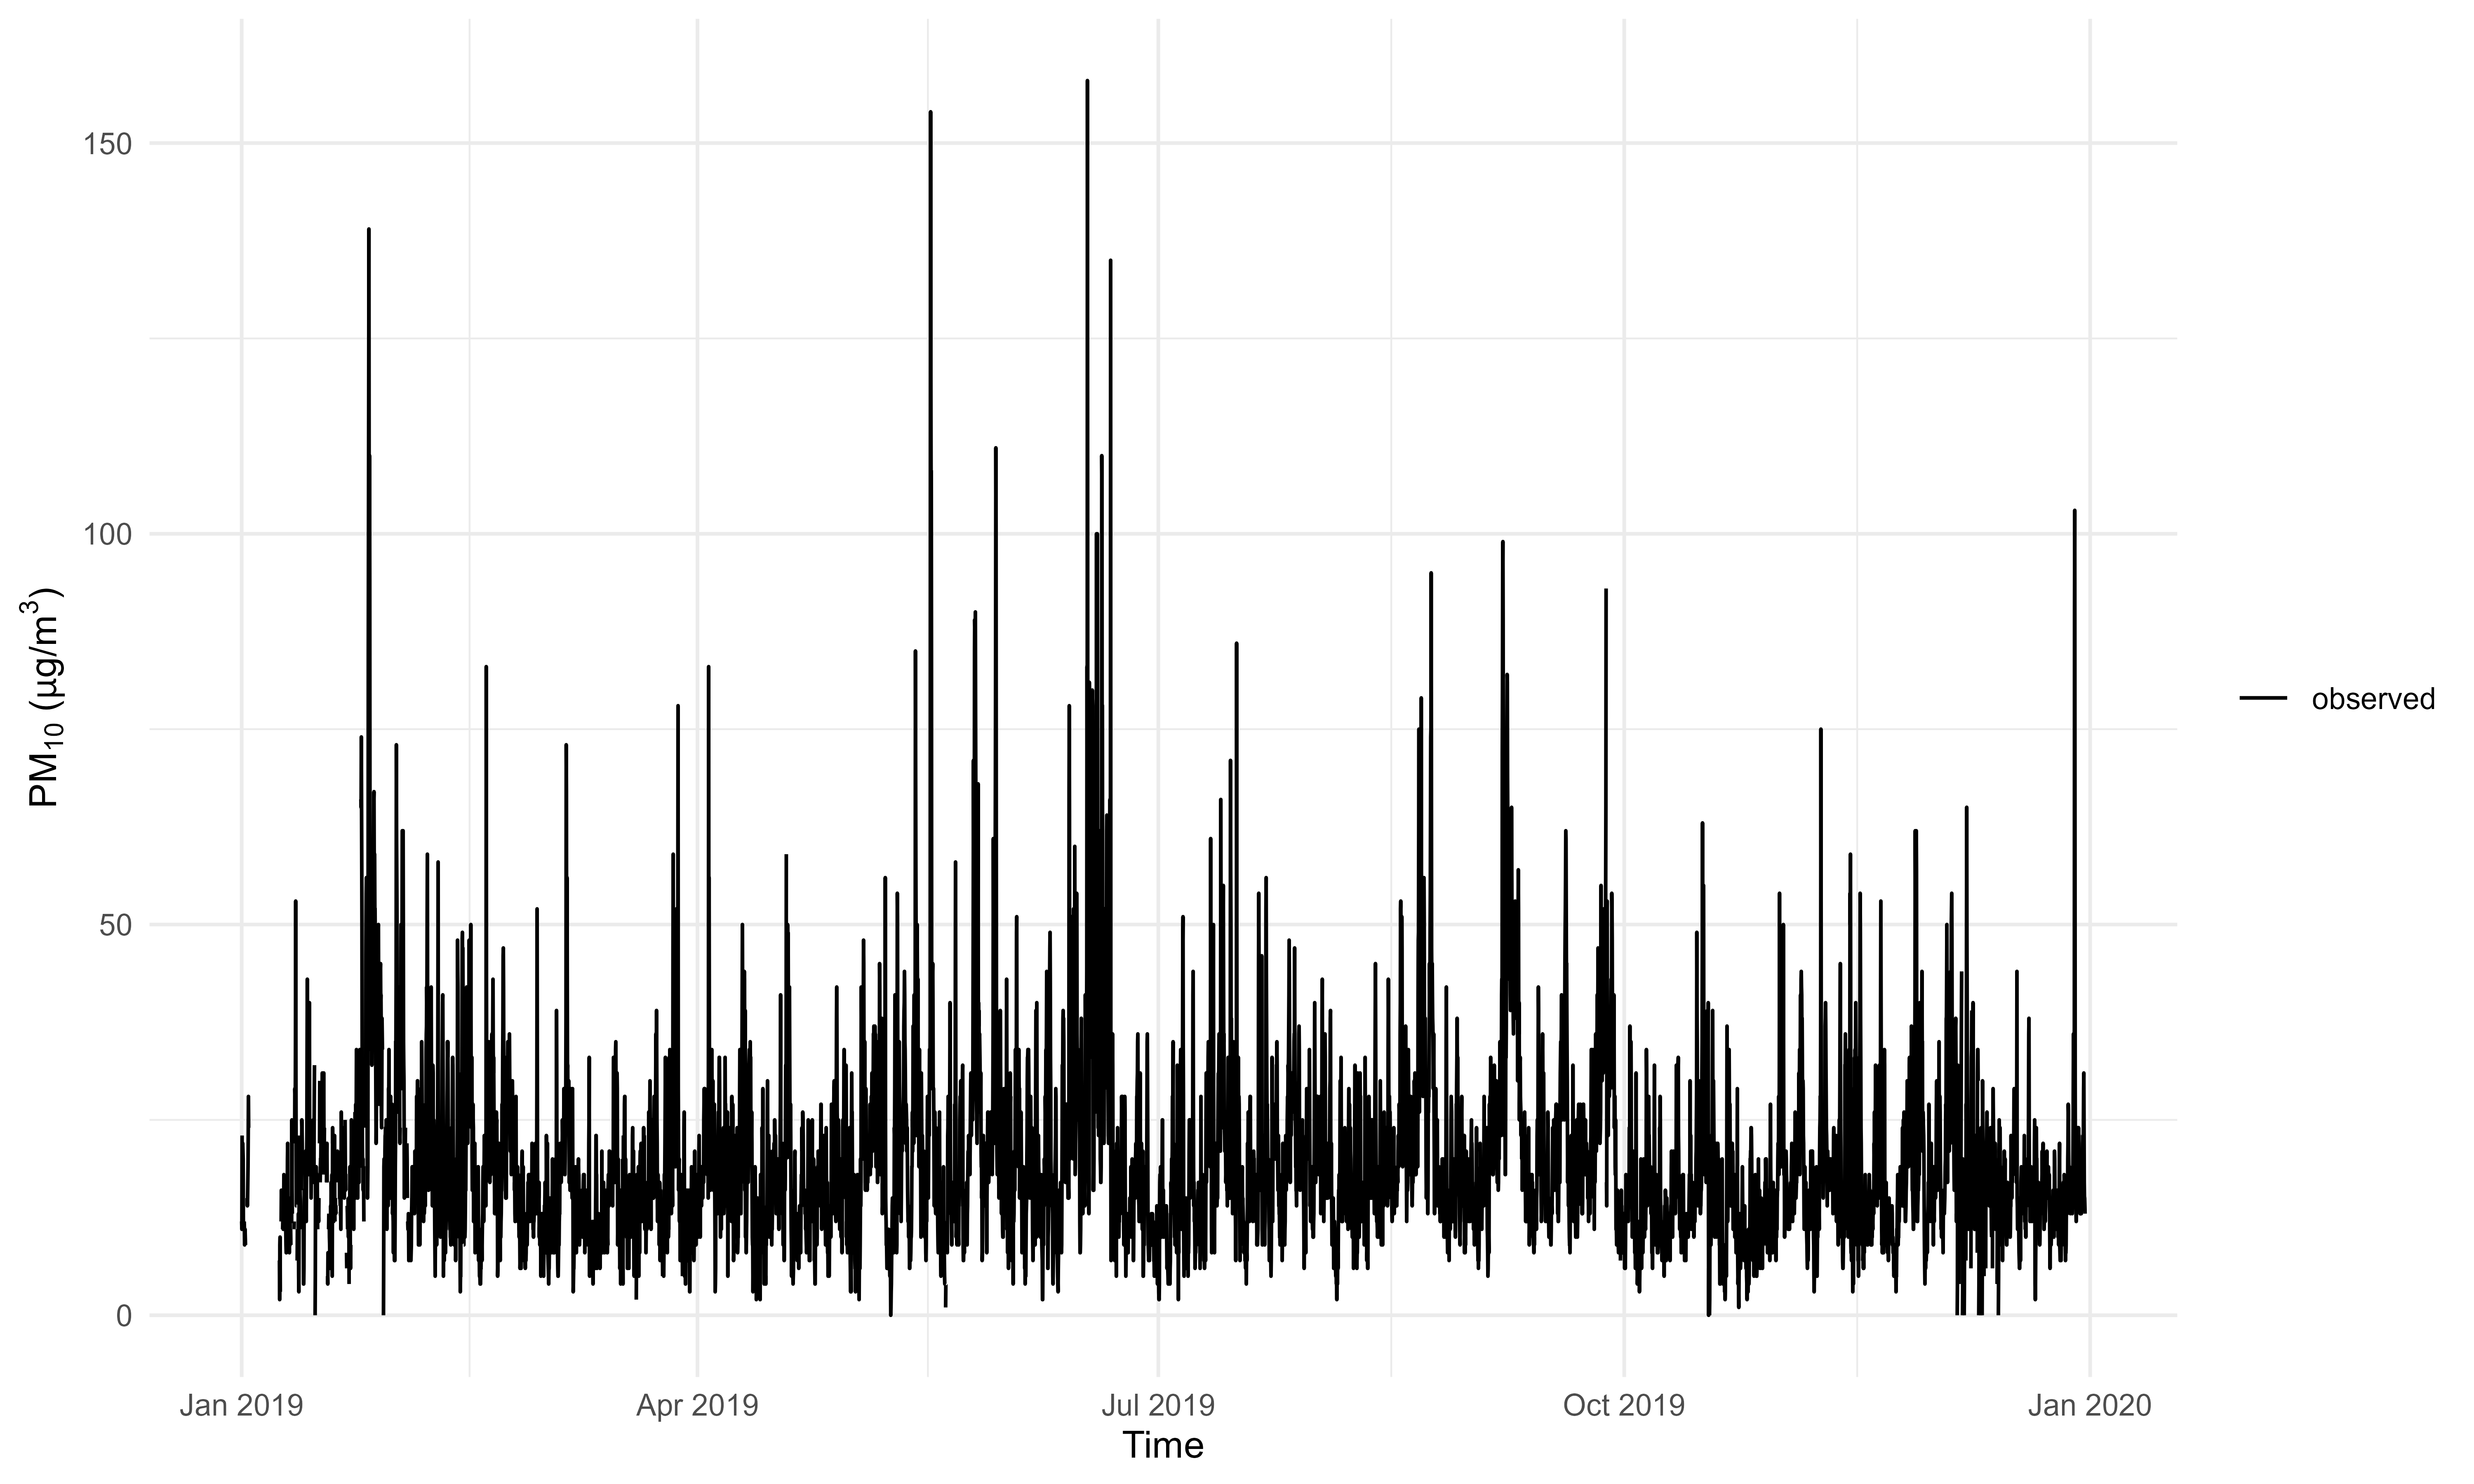
\includegraphics[width=\linewidth]{../images/extracted_data_pm10.png}
               \caption{Particulate matter 10}
            \end{subfigure}
            
            \vspace{0.5em}

            \begin{subfigure}{0.48\linewidth}
               \centering
               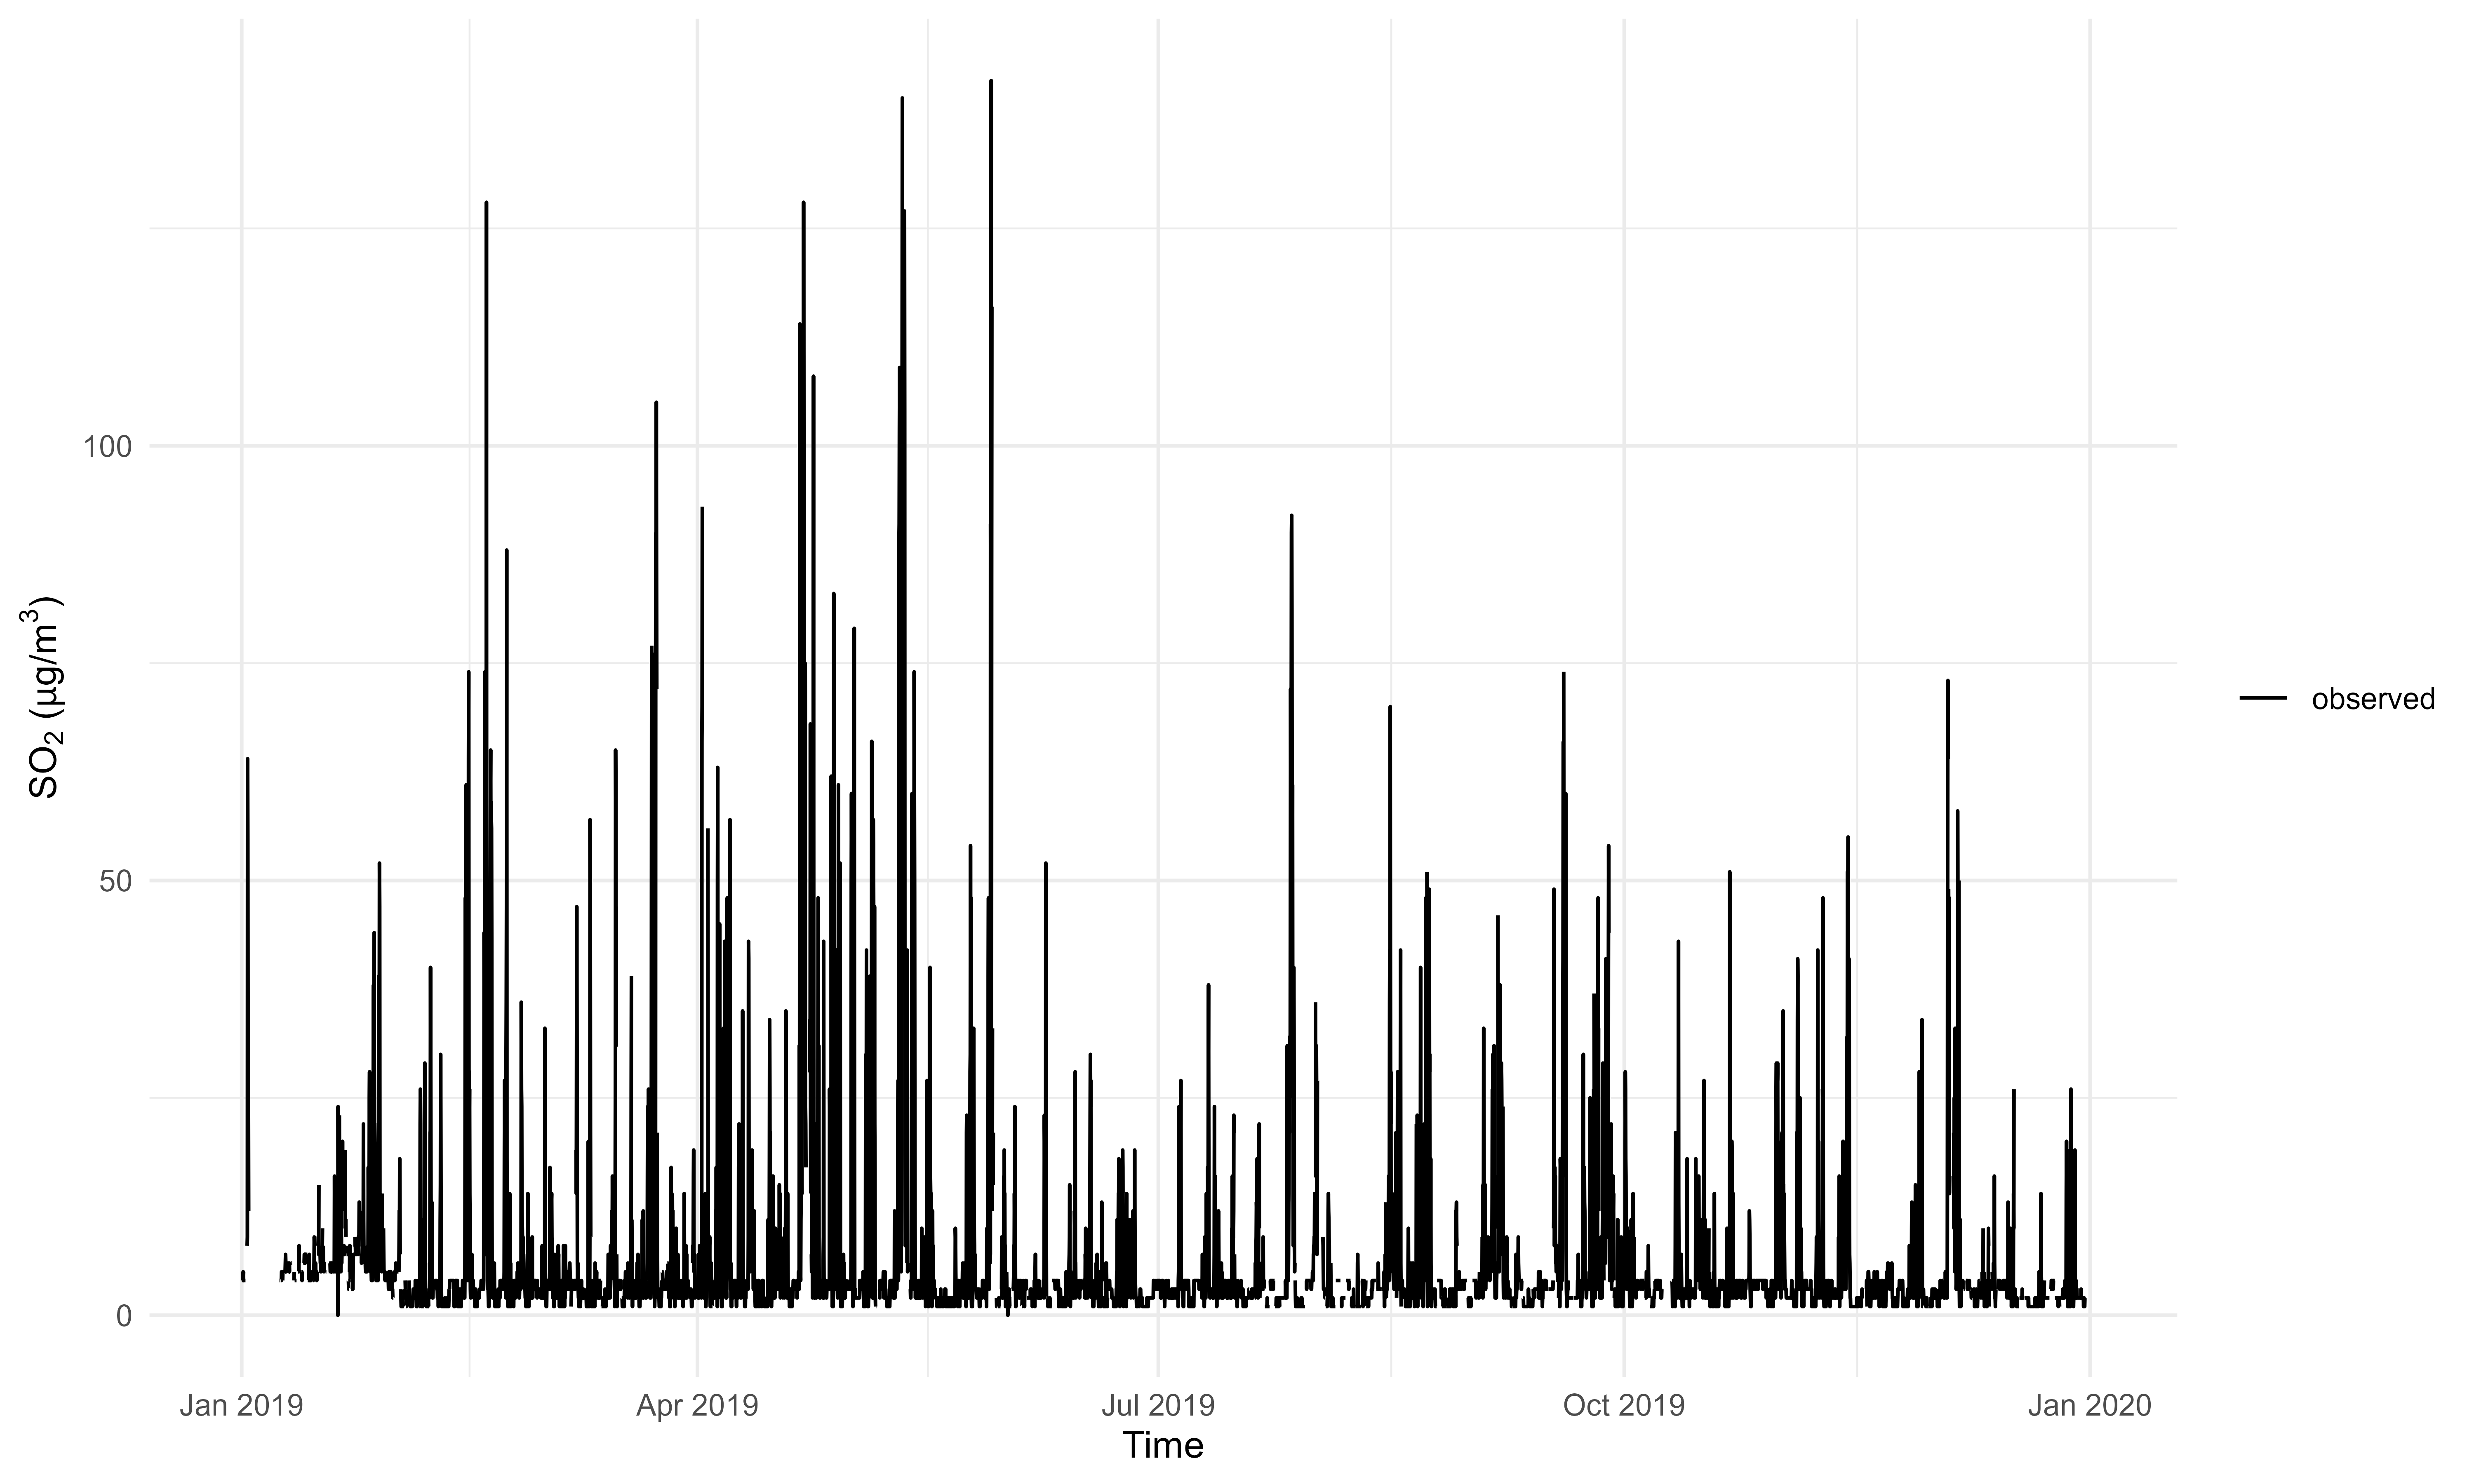
\includegraphics[width=\linewidth]{../images/extracted_data_so2.png}
            \caption{Sulphur dioxide}
            \end{subfigure}
            \hfill
            \begin{subfigure}{0.48\linewidth}
               \centering
               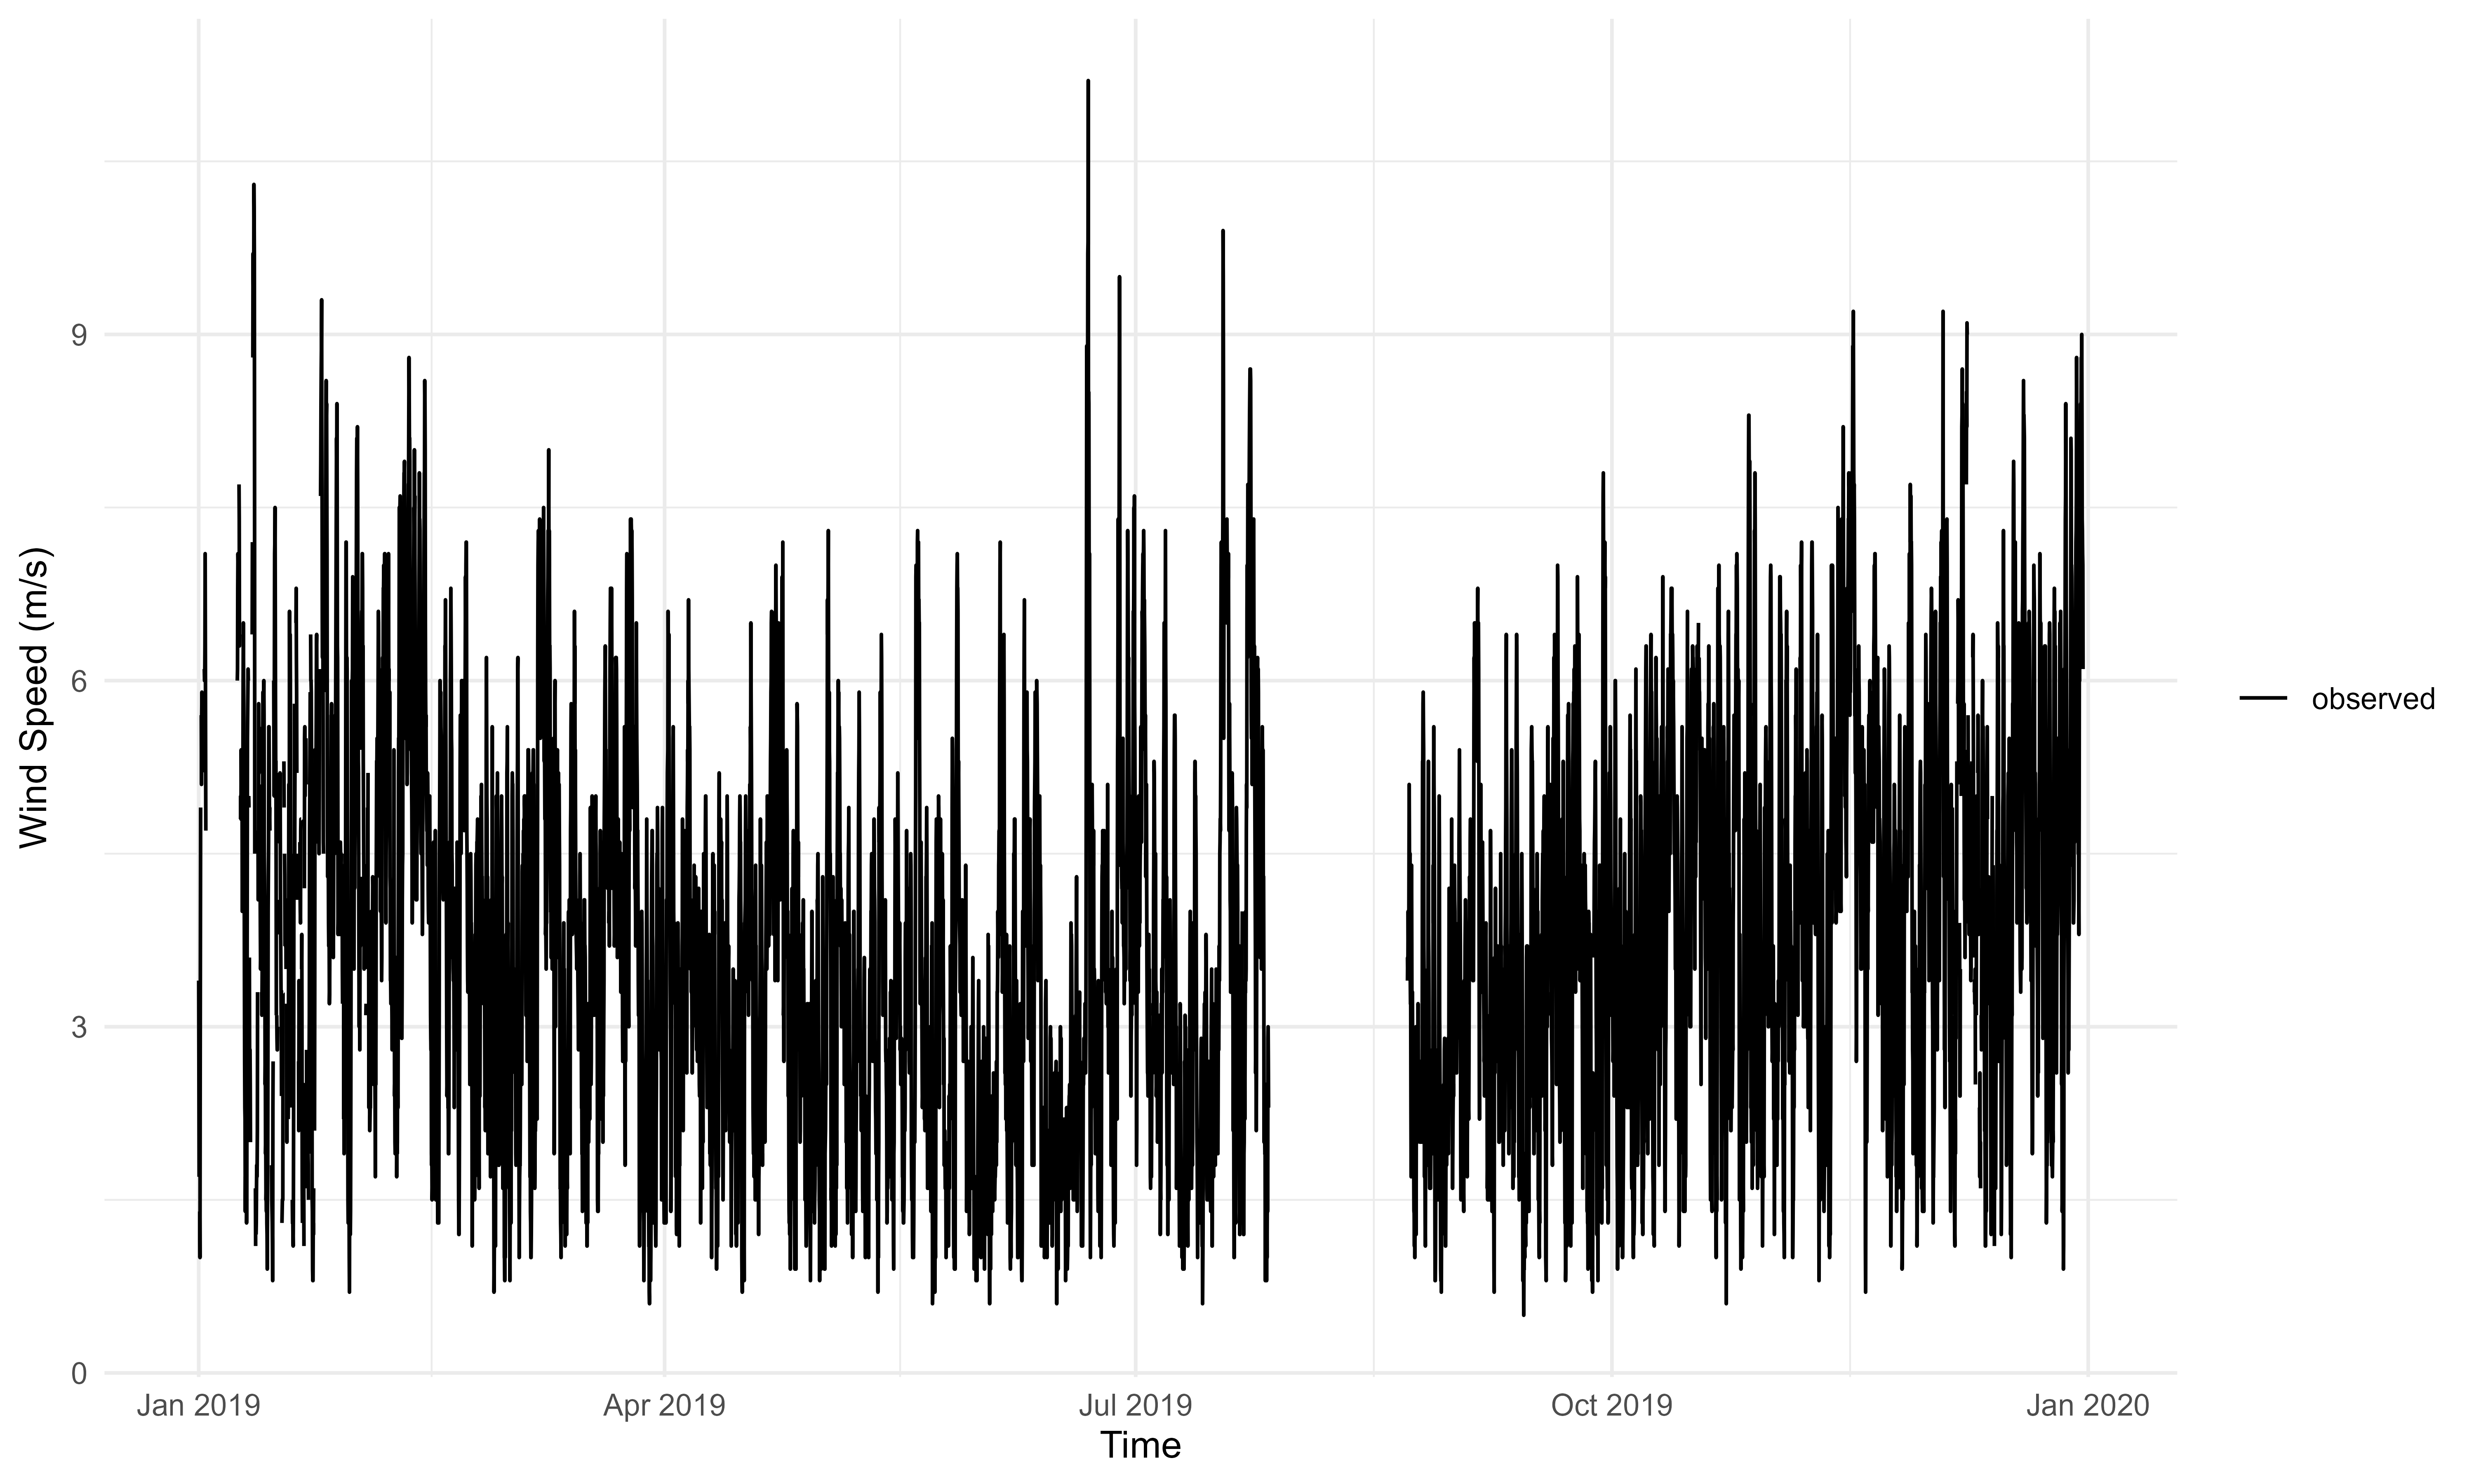
\includegraphics[width=\linewidth]{../images/extracted_data_speed.png}
               \caption{Wind speed}
            \end{subfigure}

            \caption{\textit{Time-series plots of nitrogen dioxide and meteorological processes from 01/01/2018 to 31/12/2019 measured hourly. Similar cyclic patterns can be observed in the meteorological processes, and a weaker seasonality component can be noted in the yearly nitrogen dioxide processes.}}
         \end{figure}

         There seems to be a weak seasonal and trend component based on the time series plots. There is no clear indication of a cyclical component. There is random variation as usual. It is challenging to visually identify the time series components since this is a noisy dataset.
      
         \begin{figure}[H]
            \centering
            \begin{subfigure}{0.48\linewidth}
               \centering
               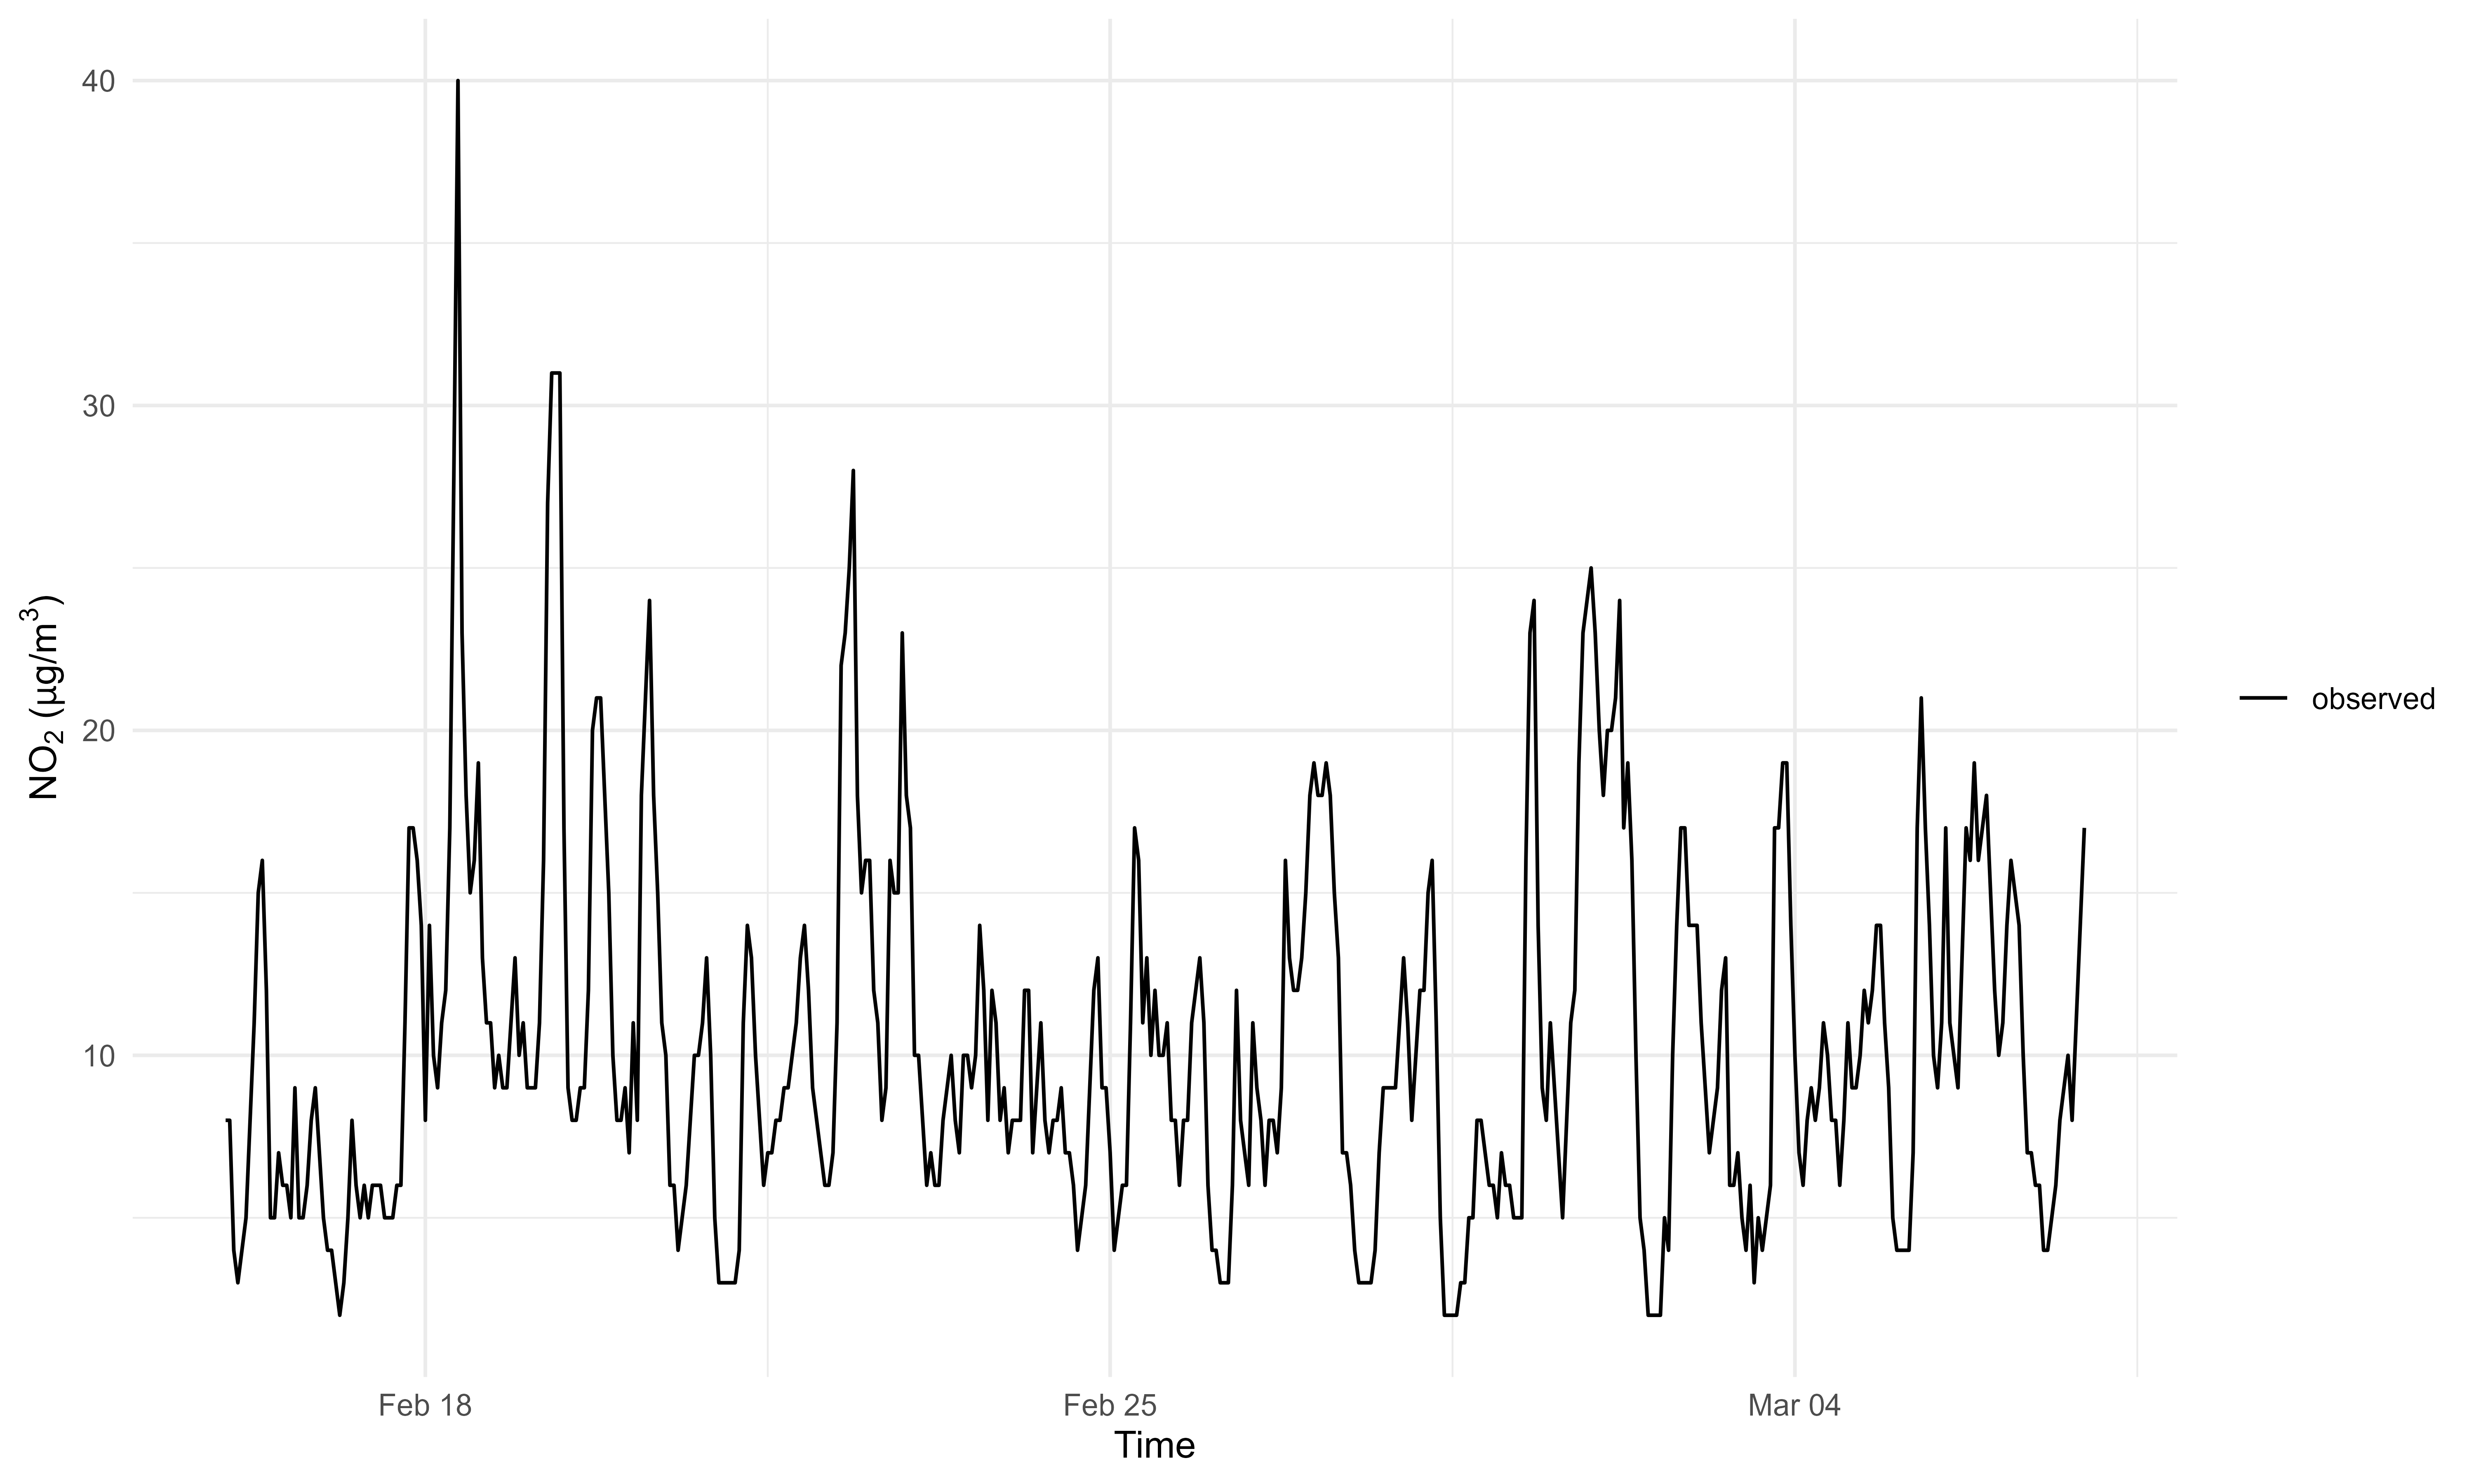
\includegraphics[width=\linewidth]{../images/subset_data_no2.png}
            \caption{Nitrogen dioxide}
            \end{subfigure}
            \hfill
            \begin{subfigure}{0.48\linewidth}
               \centering
               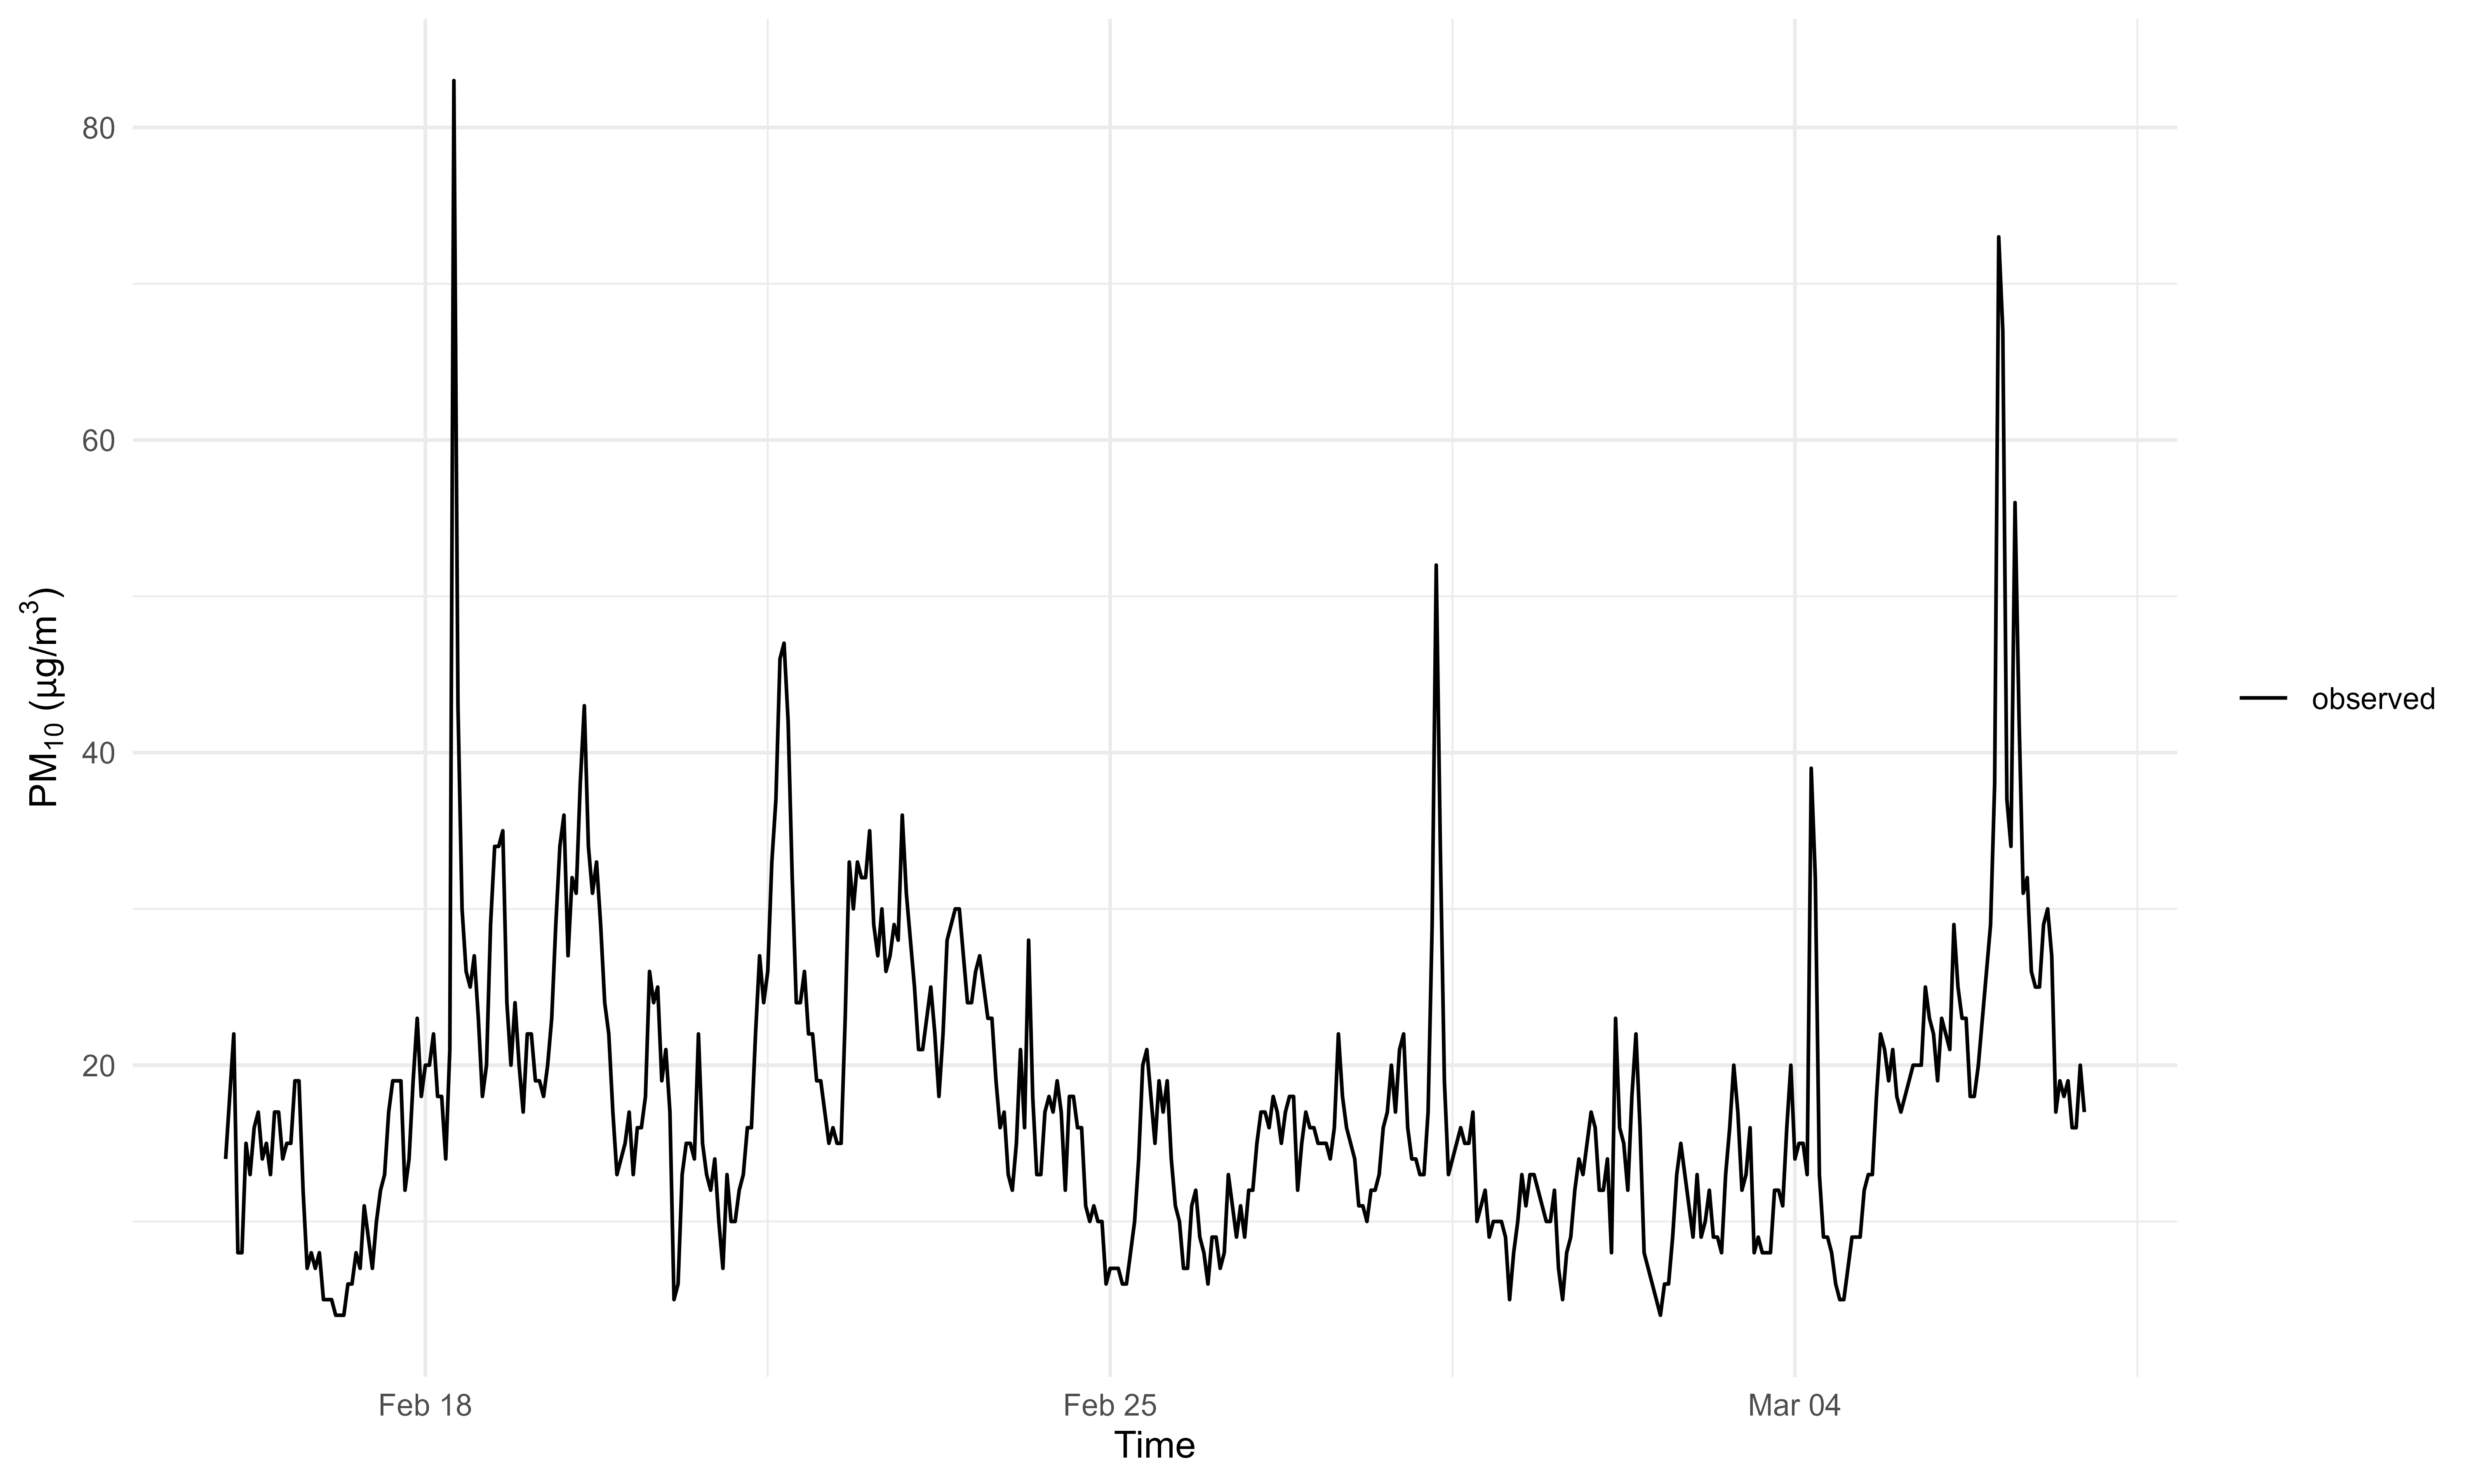
\includegraphics[width=\linewidth]{../images/subset_data_pm10.png}
               \caption{Particulate matter 10}
            \end{subfigure}
            
            \vspace{0.5em}

            \begin{subfigure}{0.48\linewidth}
               \centering
               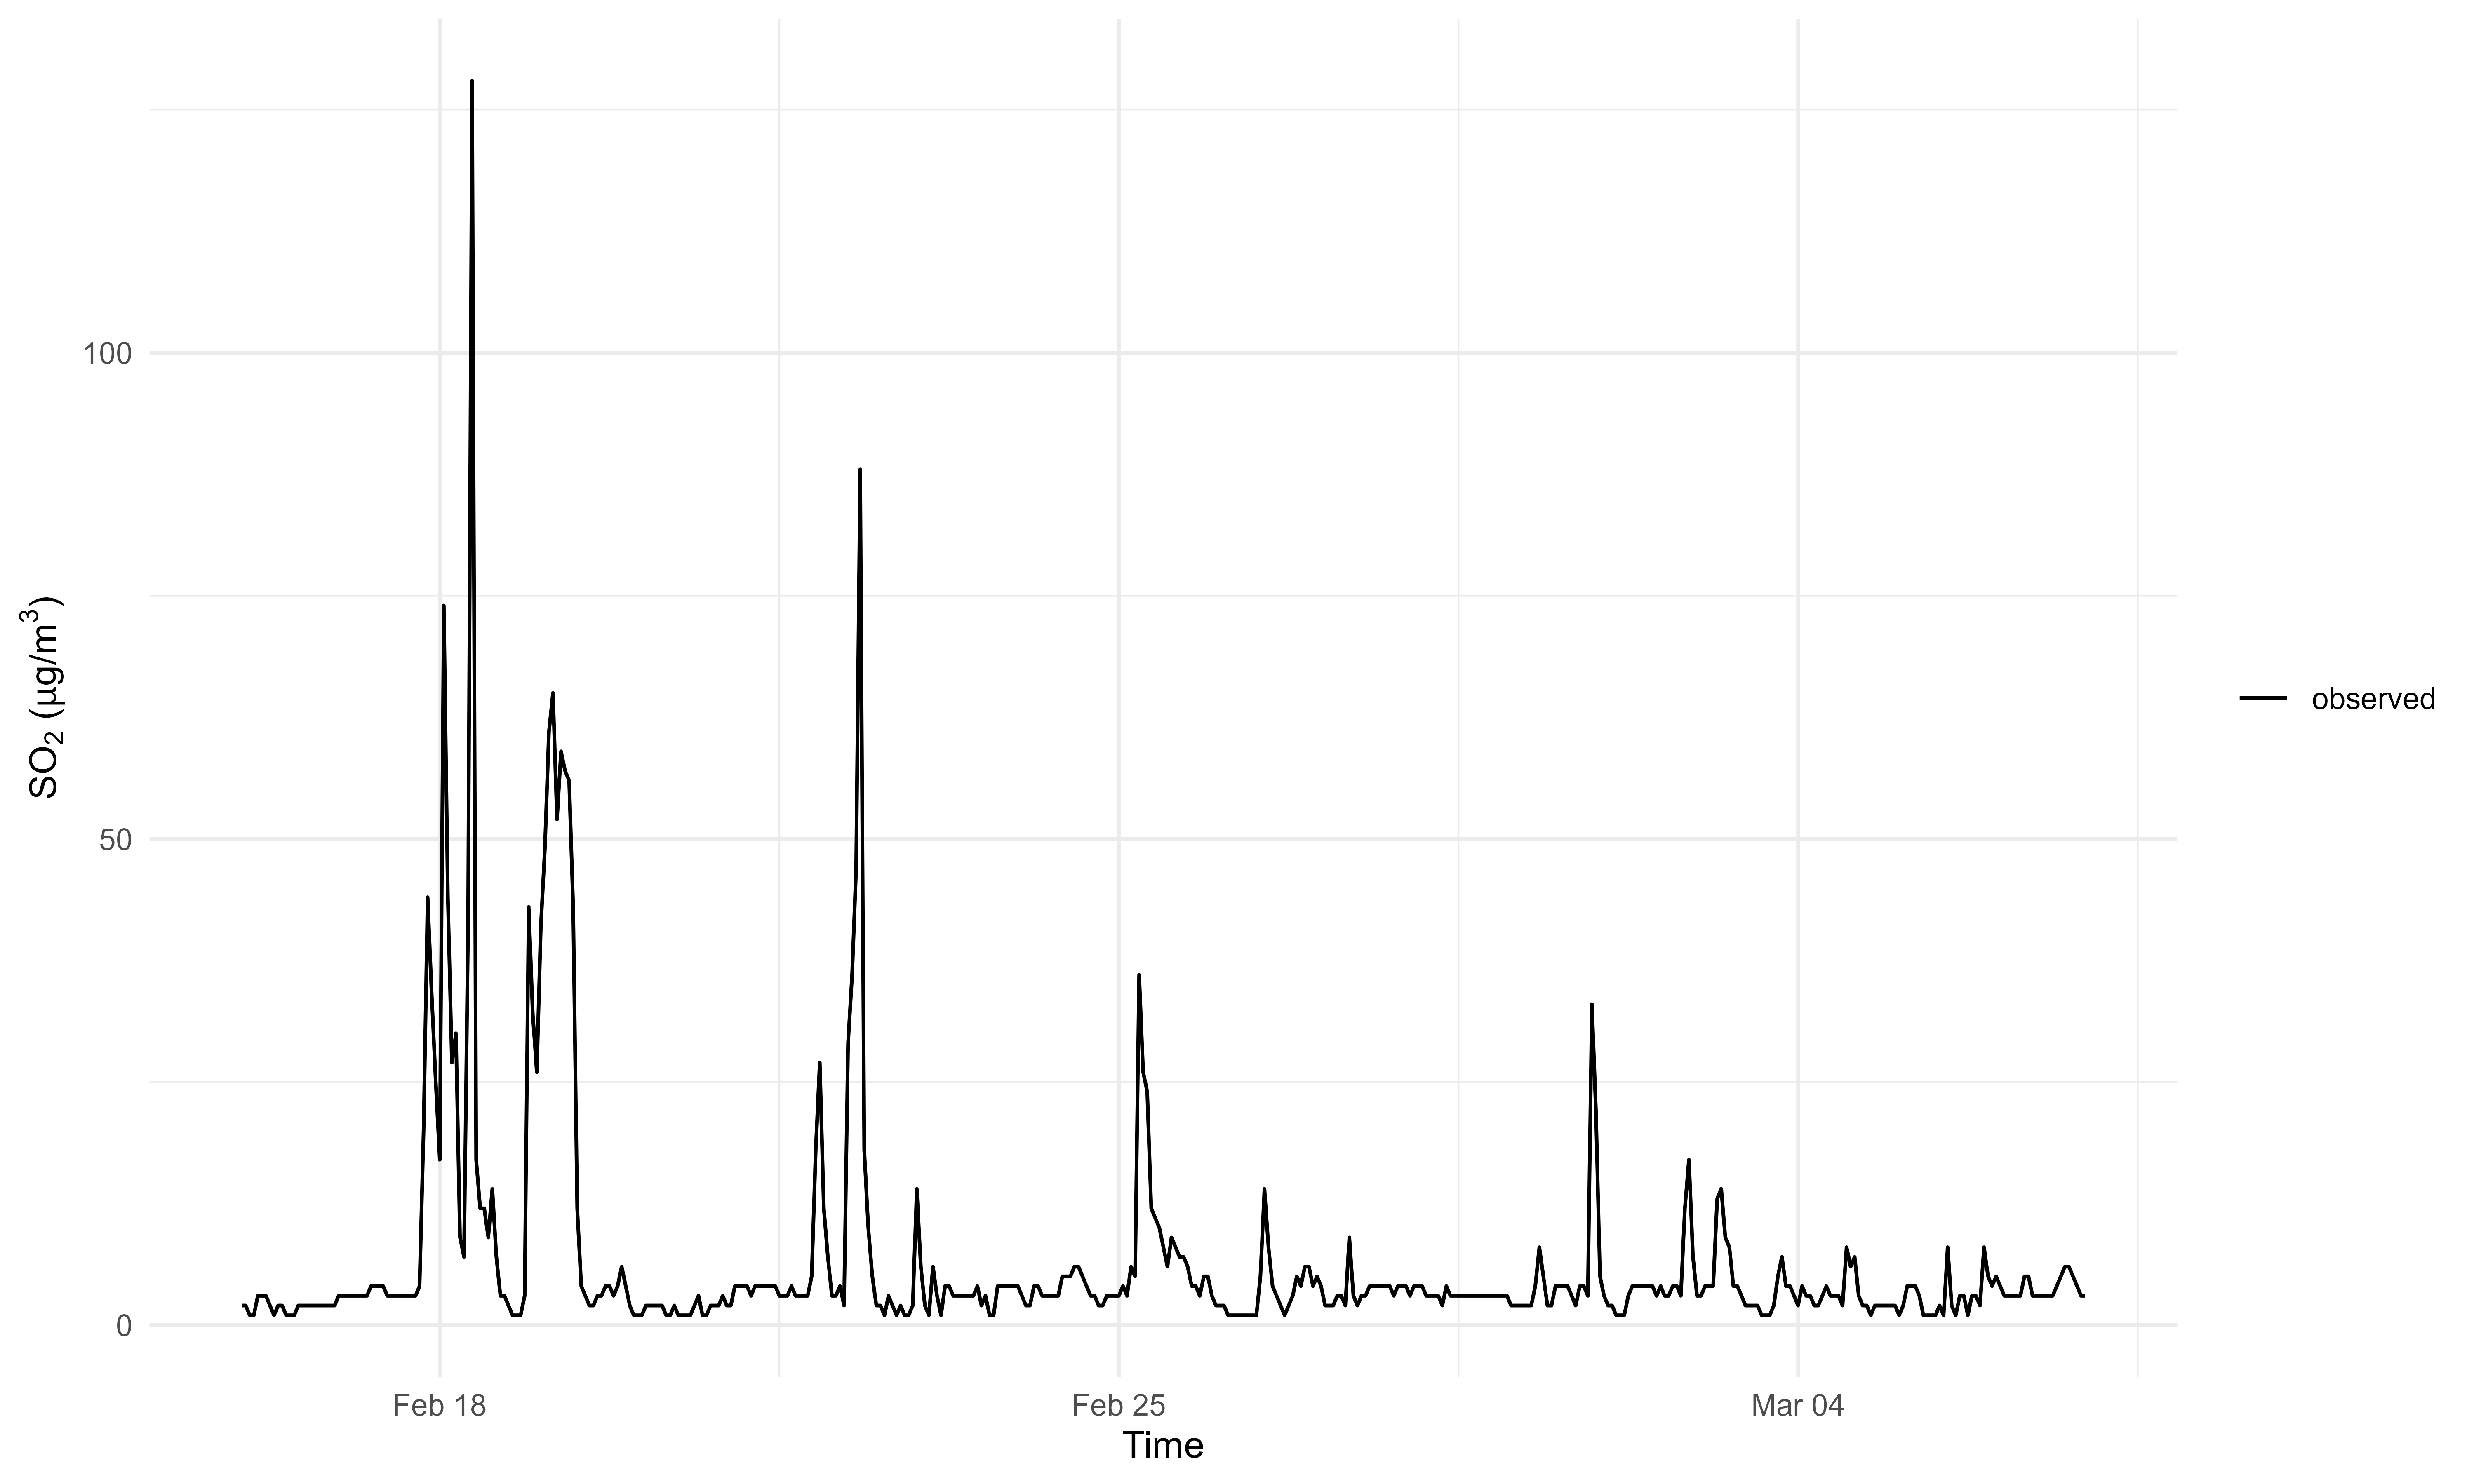
\includegraphics[width=\linewidth]{../images/subset_data_so2.png}
            \caption{Sulphur dioxide}
            \end{subfigure}
            \hfill
            \begin{subfigure}{0.48\linewidth}
               \centering
               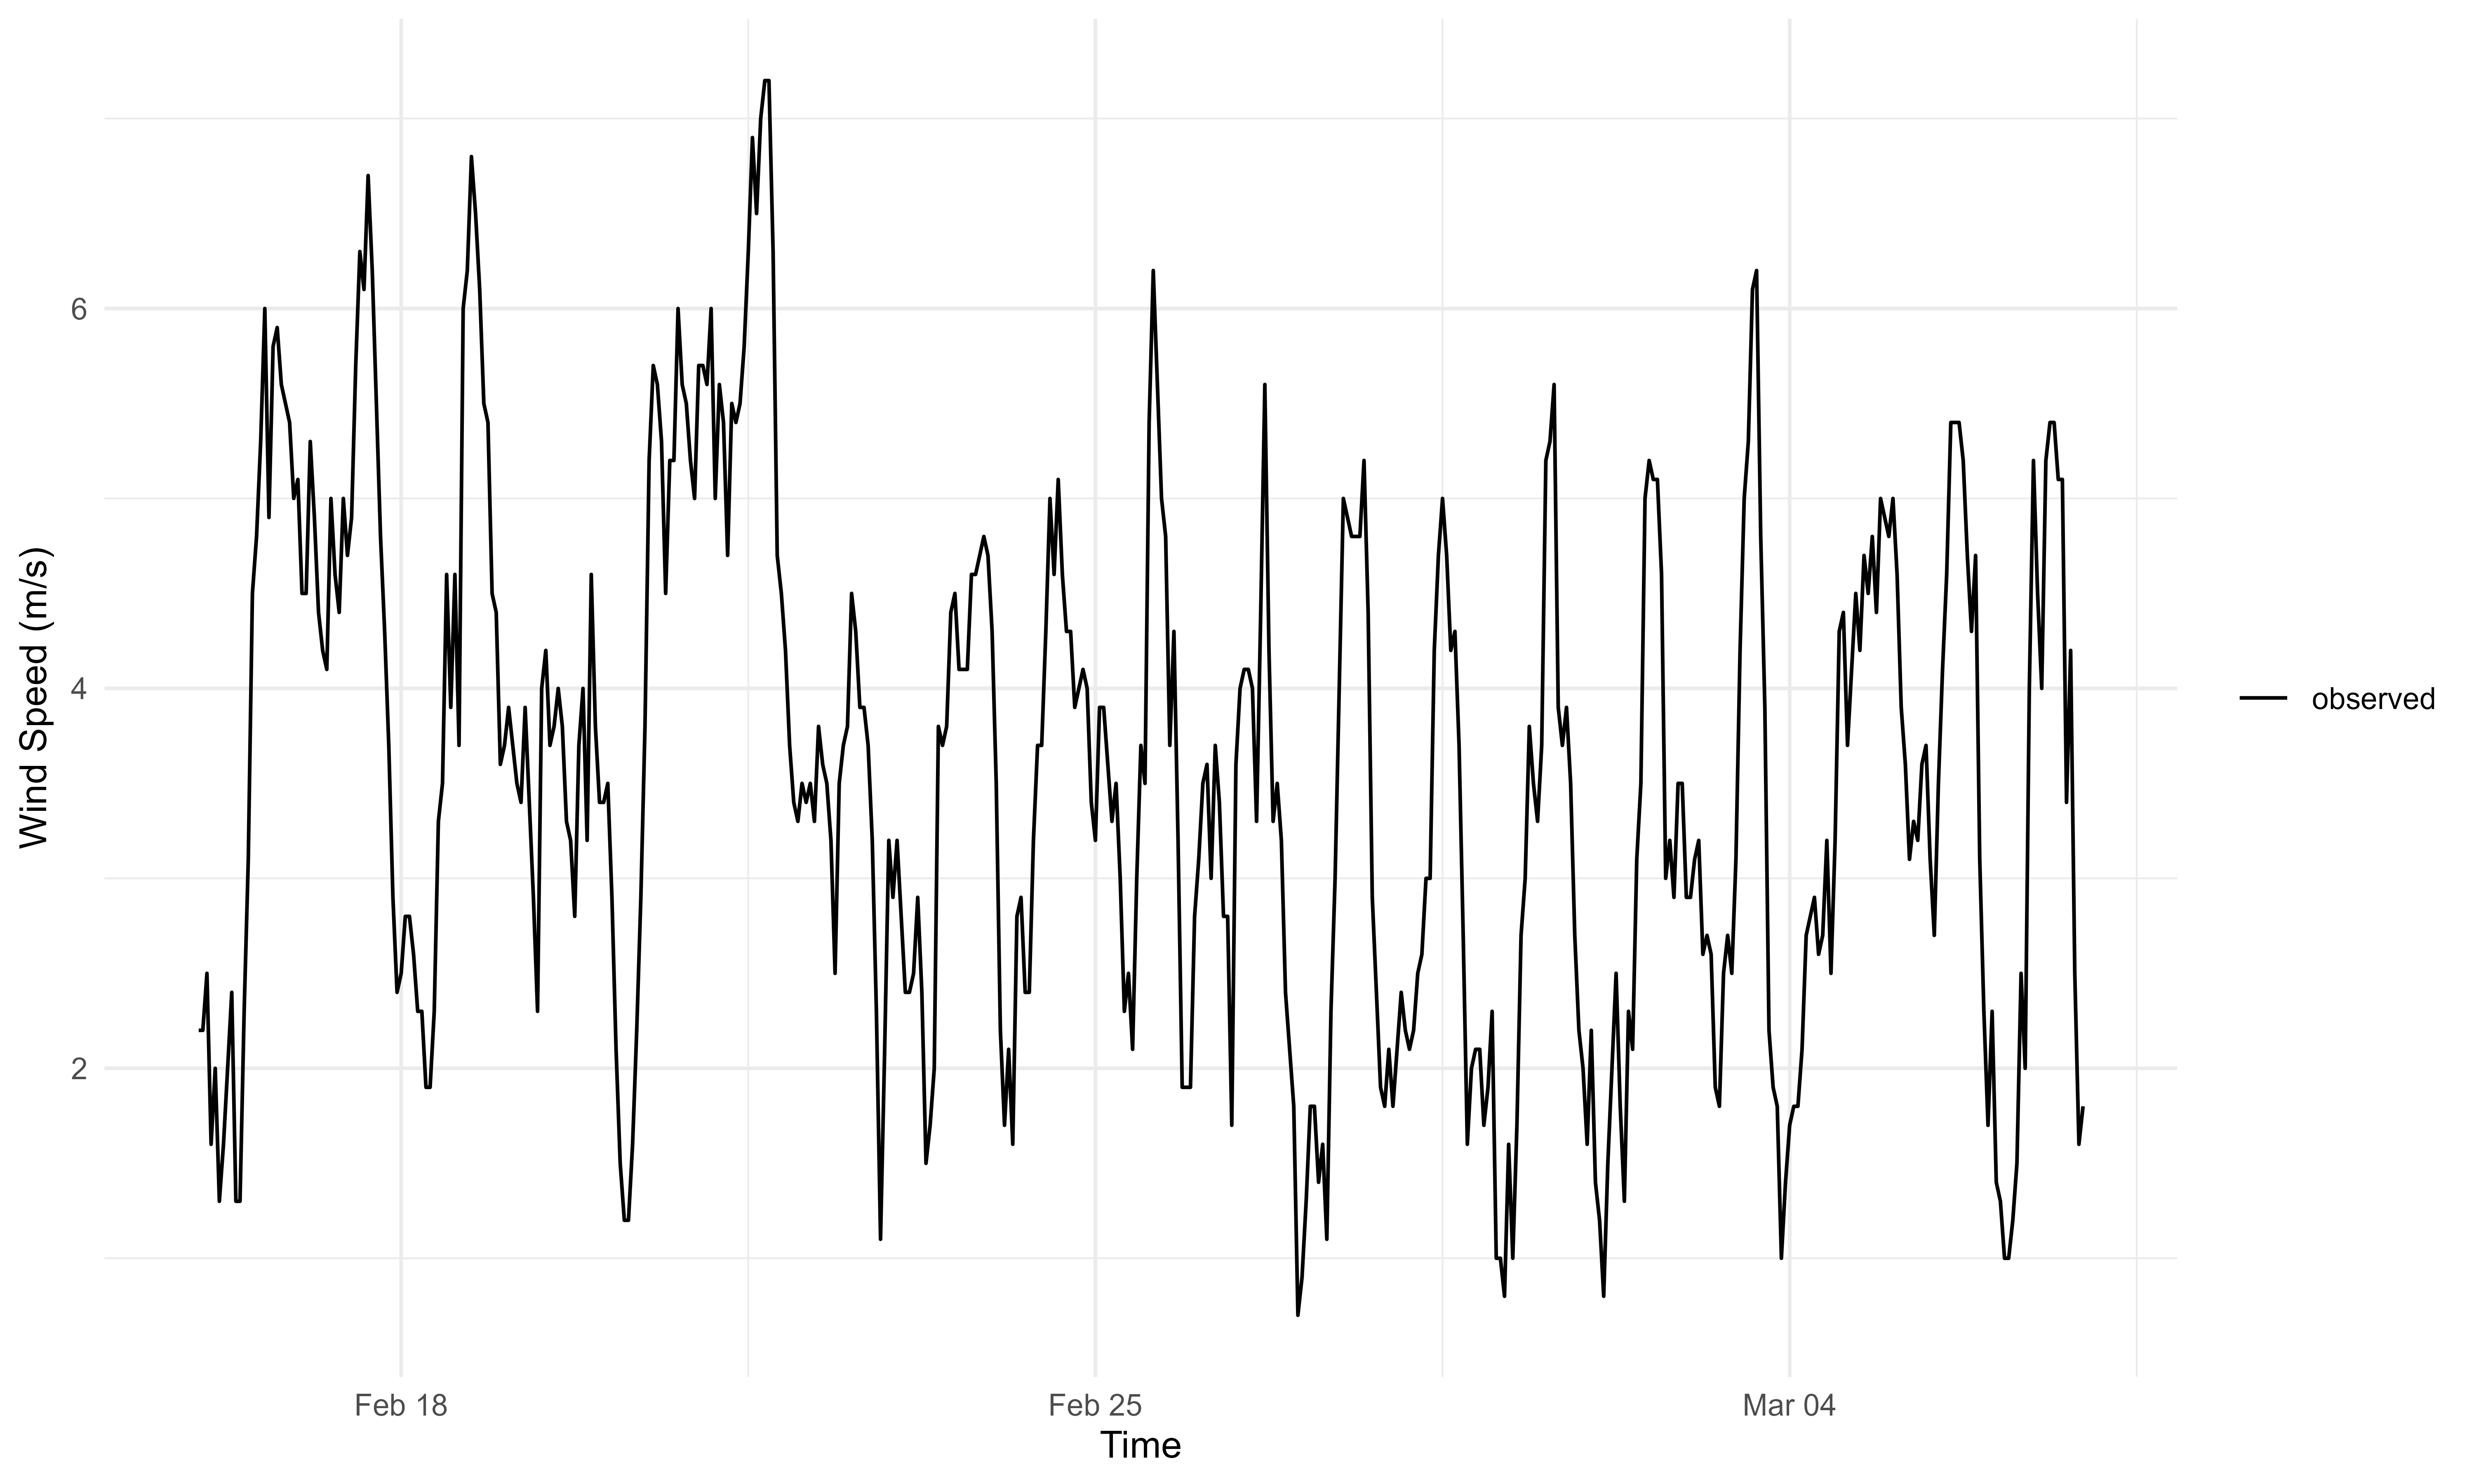
\includegraphics[width=\linewidth]{../images/subset_data_speed.png}
               \caption{Wind speed}
            \end{subfigure}

            \caption{\textit{Time-series plots of nitrogen dioxide and meteorological processes from 15/02/2019 at 23:00:00 to 06/03/2019 at 23:00:00 measured hourly. Similar cyclic patterns can be observed in the meteorological processes, and a weaker seasonality component can be noted in the yearly nitrogen dioxide processes.}}
         \end{figure}

   \subsection{Methodology}
   
      $$y \sim \text{GP}(m(\cdot),\, k(\cdot,\, \cdot))$$

      Linear mean function:

      $$m(x_{i}) = \sum_{j=1}^{p} x_{ij}\beta_{j}, \quad \text{where} \quad i \in \{1,\, \ldots,\, \text{n}\}.$$

      The resulting mean vectors of the training set and test set respectively are as follows.

      $$\mathbf{m}_{1} = \mathbf{X}_{1}\boldsymbol{\beta}$$
      $$\mathbf{m}_{2} = \mathbf{X}_{2}\boldsymbol{\beta}$$
      Squared-exponential kernel:
      $$k(x_{i},\, x_{j}) = \alpha^2 \text{exp} \bigg(-\frac{(x_{i} - x_{j})^2}{2\rho^2} \bigg) + \delta\text{I}_{i=j}, \, \text{where} \, \alpha,\, \rho \text{ are hyperparameters and } \delta = 1\text{e}-9.$$
      The resulting covariance matrices are as follows
      $$\mathbf{K}_{11} = k(\mathbf{X}_{1},\, \mathbf{X}_{1}) + \delta\mathbf{I}_{n_{1}}$$
      $$\mathbf{K}_{12} = k(\mathbf{X}_{1},\, \mathbf{X}_{2})$$
      $$\mathbf{K}_{22} = k(\mathbf{X}_{2},\, \mathbf{X}_{2}) + \delta\mathbf{I}_{n_{2}}$$
      The likelihood is the following.
      $$\mathbf{y}_{1}|\, \boldsymbol{\beta}, \alpha, \rho \sim \mathcal{N}(\mathbf{m}_{1},\, \mathbf{K}_{11})$$

      Choosing the following priors.
      $$\boldsymbol{\beta} \sim \mathcal{N}(0,\, \mathbf{I}_{p})$$
      $$\alpha \sim \text{half-normal}(0, 1)$$
      $$\rho \sim \text{half-normal}(24,\, 12)$$
      The joint distribution of $[\mathbf{y}_{1},\, \mathbf{y}_{2}]$ given fixed parameters $(\boldsymbol{\beta},\, \alpha,\, \rho)$, the joint distribution of the training and set outputs is a multivariate normal:
      $$\begin{bmatrix} \mathbf{y}_{1} \\ \mathbf{y}_{2} \end{bmatrix} \sim \mathcal{N} \Bigg(\begin{bmatrix} \mathbf{m}_{1} \\ \mathbf{m}_{2} \end{bmatrix},\, \begin{bmatrix} \mathbf{K}_{11} & \mathbf{K}_{12} \\ \mathbf{K}_{21} & \mathbf{K}_{22} \end{bmatrix} \Bigg).$$
      The conditional distribution of $\mathbf{y}_{2}|\, \mathbf{y}_{1},\, \boldsymbol{\beta},\, \alpha,\, \rho$. This is just a conditional distribution of a multivariate normal distribution which is a well known result.
      $$\mathbf{y}_{2}|\, \mathbf{y}_{1},\, \boldsymbol{\beta},\, \alpha,\, \rho \sim \mathcal{N}(\mathbf{m}_{2} + \mathbf{K}_{12}^{\text{T}}\mathbf{K}_{11}^{-1}(\mathbf{y}_{1} - \mathbf{m}_{1}),\, \mathbf{K}_{22} - \mathbf{K}_{12}^{\text{T}} \mathbf{K}_{11}^{-1} \mathbf{K}_{12})$$
      $$\pi(\mathbf{y}_{2}|\, \mathbf{y}_{1}) = \int \pi(\mathbf{y}_{2}|\, \mathbf{y}_{1},\, \boldsymbol{\beta},\, \alpha,\, \rho) \, \pi(\boldsymbol{\beta}) \, \pi(\alpha) \, \pi(\rho) \,  d\boldsymbol{\beta}\, d\alpha\, d\rho.$$
      This does not have a closed form solution. We approximated the posterior samples of this distribution using `Stan`. `Stan` avoids computing explicit inverses. These quantities are calculated in `Stan` as follows.

      Cholesky decomposition of $\mathbf{K}_{11}$. 
      $$\mathbf{K}_{11} = \mathbf{L} \mathbf{L}^{\text{T}}.$$

      Compute $\mathbf{w} = \mathbf{K}_{11}^{-1}(\mathbf{y}_{1} - \mathbf{m}_{1})$ via triangular solves:
      $$\mathbf{v} = \mathbf{L}^{-1}(\mathbf{y}_{1} - \mathbf{m}_{1}).$$
      Then $$\mathbf{w} = (\mathbf{L}^{\text{T}})^{-1} \mathbf{v}.$$
      Thus $$\mathbf{w} = \mathbf{K}_{11}^{-1}(\mathbf{y}_{1} - \mathbf{m}_{1}).$$

      The predictive mean is calculated as follows. 

      $$\mathbf{m}_{2} + \mathbf{K}_{12}^{\text{T}}\mathbf{w} = \mathbf{m}_{2} + \mathbf{K}_{12}^{\text{T}}\mathbf{K}_{11}^{-1}(\mathbf{y}_{1} - \mathbf{m}_{1}).$$
      And the predictive covariance is calculated as follows.

      $$\mathbf{A} = \mathbf{L}^{-1} \mathbf{K}_{12}.$$
      Then $$\mathbf{A}^{\text{T}} \mathbf{A} = \mathbf{K}_{12}^{\text{T}} \mathbf{L}^{-\text{T}} \mathbf{L}^{-1} \mathbf{K}_{12}.$$
      Thus $$\mathbf{A}^{\text{T}} \mathbf{A} = \mathbf{K}_{12}^{\text{T}} \mathbf{K}_{11}^{-1} \mathbf{K}_{12}.$$

      Then draw samples from $\mathbf{y}_{2}|\, \mathbf{y}_{1}$ via Hamiltonian Monte Carlo (HMC) in `Stan`. The algorithm proceeds as follows.

      1. `Stan` samples the parameters $(\boldsymbol{\beta},\, \alpha,\, \rho)$ from the posterior distribution $\pi(\boldsymbol{\beta},\, \alpha,\, \rho|\, \mathbf{y}_{1})$ using HMC.

      2. For each parameter draw `Stan` then executes the `generated quantities` block which:
      - Computes the predictive mean and predictive covariance,
      - draws $$\mathbf{y}_{2}^{(s)} \sim \mathcal{N}(\text{pred mean},\, \text{pred covariance})$$ using `multi_normal_rng`. 
         The RNG draw is not part of the HMC dynamics - it happens after the sampler proposes/accepts a parameter sample.

      3. Collecting the $\mathbf{y}_{2}^{(s)}$ across all saved iterations gives a Monte Carlo approximation to the marginal posterior predictive $$\pi(\mathbf{y}_{2}|\, y_{1}) \approx \frac{1}{S} \sum_{s=1}^{S} \mathcal{N}(\mathbf{y}_{2}|\, \mu^{(s)},\, \Sigma^{(s)}),$$ where $\mu^{(s)},\, \Sigma^{(s)}$ are conditional mean/covariance computed at the $s$-th parameter draw.
   
   \subsection{Cross-validation}

      Cross-validation was conducted as follows: a period of 7 days from 08/02/2019 at 00:00 to 15/02/2019 at 23:00 was used for the training set, and 1 day from 16/02/2019 at 00:00 to 16/02/2019 23:00 was used as a test set. On each iteration, we increment the training set by 1 day and shift the test set by 1 day, after which loss functions (MSE, MAE, and MAPE) are calculated and stored in a matrix. Once all 1 iterations are completed, the error functions are averaged over all iterations.

      \begin{figure}[H]
            \centering
            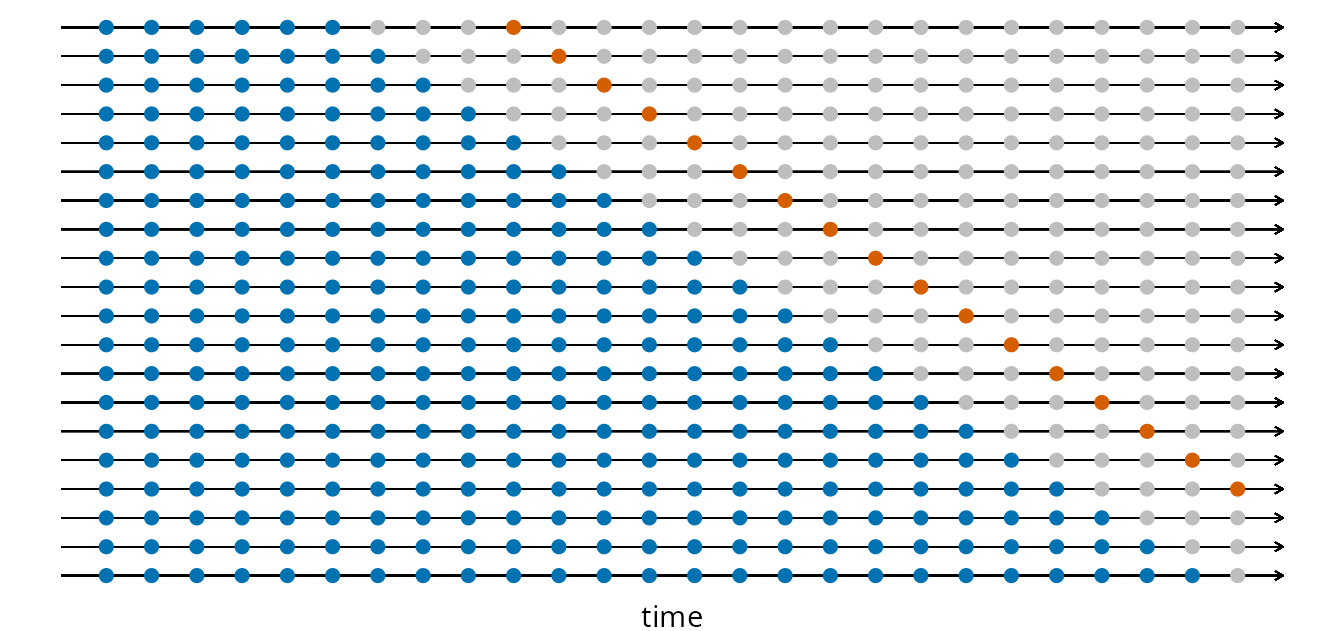
\includegraphics[width=0.48\linewidth]{../images/cross_validation.png}
            \caption{\textit{Illustration of the rolling-origin cross-validation scheme, showing the expanding training set and one-step-ahead test set. \cite{fpp3_CV}}}
      \end{figure}
   
   \subsection{Results}

      \begin{table}[H]
         \centering
         \begin{tabular}{lcccccc}
         \hline
         \multirow{2}{*}{Model} & \multicolumn{3}{c}{RMSE} & \multicolumn{3}{c}{MAE} \\
         \cline{2-7}
         & \multicolumn{3}{c}{Forecasts} & \multicolumn{3}{c}{Forecasts} \\
         & \multicolumn{3}{c}{($h$ day time horizon)} & \multicolumn{3}{c}{($h$ day time horizon)} \\
         & 24 & 168 & 744 & 24 & 168 & 744 \\
         \hline
         Average & {7.731} & \textbf{\textcolor{red}{5.397}} & {7.439} & \textbf{\textcolor{red}{6.042}} & \textbf{\textcolor{red}{4.254}} & {5.385} \\
         Naive & {10.553} & {7.864} & {10.040} & {7.708} & {6.071} & {7.308} \\
         Drift & {10.606} & {8.128} & {11.358} & {7.764} & {6.391} & {8.809} \\
         AR(1) & {8.662} & {5.912} & {8.044} & {6.029} & {4.422} & {5.616} \\
         GP-0-WN & {13.756} & {11.141} & {13.169} & {11.719} & {9.786} & {11.081} \\
         GP-0-SE & {~} & {~} & {~} & {~} & {~} & {~} \\
         GP-MLR-WN & \textbf{\textcolor{red}{7.692}} & {6.134} & \textbf{\textcolor{red}{7.225}} & {6.119} & {4.490} & \textbf{\textcolor{red}{5.136}} \\
         GP-MLR-SE & {~} & {~} & {~} & {~} & {~} & {~} \\
         \hline
         \end{tabular}
         \caption{\textit{RMSE and MAE of forecasting models across horizons.}}
      \end{table}
